\documentclass[fontset=fandol, zihao=-4]{ctexart}
\linespread{1.5}
\usepackage[a4paper, scale=0.75]{geometry}
\usepackage{amsmath,amssymb,amsfonts}
\numberwithin{equation}{section}    % let the equation number displays in (1.1) style
\numberwithin{figure}{section}
\usepackage{unicode-math}
\setmathfont{STIX2Math}[Extension={.otf}, Path=./STIX2fonts/, Scale=1]
\setmainfont{STIX2Text}[Extension={.otf}, Path=./STIX2fonts/, UprightFont={*-Regular}, BoldFont={*-Bold}, ItalicFont={*-Italic}, BoldItalicFont={*-BoldItalic}]
\usepackage{graphicx}
\usepackage{xcolor}
\usepackage{hyperref}
\usepackage{physics}    % symbols related to physics
% \usepackage{ulem}       % strikethrough \sout
\usepackage{xeCJKfntef} % for Chinese underline style
\usepackage{tcolorbox}  % colored textbox environment
\tcbuselibrary{breakable}   % tcolorbox setup
\usepackage[angle=0, scale=0.5]{draftwatermark}
\SetWatermarkText{
\includegraphics{figures/TheStarAlight_logo.png}}
\hypersetup{colorlinks=true,linkcolor=blue,citecolor=blue,urlcolor=magenta} % hyperref setup
\usepackage{caption}
\captionsetup{font+=it}     % italic (kaiti for Chinese) for captions
\renewcommand*{\thefootnote}{「\arabic{footnote}」} % change footnote style (「1」)
% shortcuts
    % color
    \newcommand{\cyan}[1]{\textcolor{cyan}{#1}}
    % math style
    \renewcommand{\rm}[1]{\mathrm{#1}}  % roman, redefining original \rm
    \newcommand{\bm}[1]{\symbfit{#1}}   % bold+italic, using \symbfit instead of conventional \bm
    \newcommand{\br}[1]{\symbf{#1}}     % bold+roman
    % math
    \newcommand{\pd}{\partial}      % partial symbol
    % \newcommand{\dd}{\mathrm{d}}  % roman d (derivative & integral) [already implemented in the physics pkg]
    \newcommand{\ii}{\mathrm{i}}    % roman i (imag.)
    \newcommand{\ee}{\mathrm{e}}    % roman e (exp)
    % \newcommand{\abs}[1]{\lvert #1 \rvert}  % abs symbol [already implemented in the physics pkg]
    \renewcommand{\Re}{\mathcal{R}} % Re symbol
    \renewcommand{\Im}{\mathcal{I}} % Im symbol
    \newcommand{\del}{\br{\nabla}}  % bold nabla symbol
    % frequently-used notations
    \newcommand{\rr}{\bm{r}}
    \newcommand{\pp}{\bm{p}}
    \newcommand{\LL}{\bm{L}}
    \renewcommand{\AA}{\bm{A}}
    \renewcommand{\dag}{\dagger}    % dagger symbol
    \newcommand{\diag}{\rm{diag}\ } % diagonal matrix notation
    \newcommand{\eps}{\varepsilon}
    \newcommand{\up}{\uparrow}
    \newcommand{\down}{\downarrow}
    % colors
    \newcommand{\blue}[1]{\textcolor{blue}{#1}}
    \newcommand{\red}[1]{\textcolor{red}{#1}}
    \newcommand{\green}[1]{\textcolor{green}{#1}}
    \newcommand{\purple}[1]{\textcolor{purple}{#1}}
    % others
    \catcode`\。=\active % replace 。with .
    \newcommand{。}{\ifmmode\text{.}\else .\fi} % replace 。with .
    \renewcommand{\emph}[1]{\CJKunderline*[textformat=\bfseries]{#1}}
    \newcommand{\schrodinger}{Schr\"{o}dinger}

\begin{document}

\title{\LARGE \textbf{量子力学期末复习}\\ \textsc{Review Notes for Quantum Mechanics}}
\author{\Large \textsc{Mingyu Zhu}}
\date{
    \today \\
    \normalsize \textit{Edition 0.3 Build 11}
}

\setcounter{page}{0}
\maketitle
\thispagestyle{empty}
\tableofcontents
\pagebreak


\section*{前言}
\markboth{前言}{前言}
\addcontentsline{toc}{section}{前言}

\pagebreak

\section{量子力学基本原理}
\label{sec:principles}

% =================================================
\subsection{不确定性原理}
\label{subsec:principles_uncertainty}

量子力学与经典力学之间的一大矛盾就在于\emph{不确定性原理}(uncertainty principle)。
在原子尺度上,经典力学的运动观念与实验的结论出现了巨大的鸿沟。
例如,在经典电动力学的框架下,围绕原子核做轨道运动的电子会释放电磁波从而最终落入原子核中;
电子衍射实验中,电子的行为呈现出波动特征(这种现象称为\emph{波粒二象性},wave-particle duality
\footnote{需要阐明的是,波粒二象性本身便可以视为不确定性原理的一项推论。}
)。

为了更准确地描述不确定性原理,我们需要明确\emph{测量}这一概念。
这里测量通常指的是一个服从经典力学的\emph{仪器}与被测量体系的相互作用,从而获得与体系有关的某个物理量的过程。
测量是理想的,这是说,我们在此不考虑仪器存在的噪声、误差等因素。

然而,不确定性原理表明,即便排除了仪器的噪声和干扰,我们所得的物理量测量结果也往往是不能用经典理论解释的。
例如,倘若我们反复测量一个低能电子的位置$\rr$,并通过逼近的手段试图求取电子的瞬时速度(即$\bm{v}=\lim_{\Delta t\rightarrow 0}\Delta\rr/\Delta t$),我们会发现所得的瞬时速度根本不收敛,
这意味着经典力学中的轨迹概念在量子力学中彻底失效了——在经典力学中,我们可以通过测量某一时刻系统的全部参数(广义坐标$q$与动量$p$),从而通过运动方程准确地预言系统之后的任何行为;而一个量子体系无法同时拥有确切的坐标和速度,因而也无法被精确预测。

不过,尽管我们无法准确预言量子体系的行为,但我们可以预言测量量子体系得到某一结果的概率(否则量子力学就要成为一门玄学了)。
这就是说,\emph{量子力学并不给出下一次测量的确切结果,而是给出测量结果的概率分布。}


% =================================================
\subsection{量子态叠加与统计诠释}
\label{subsec:principles_quantum_state}

% ================================
\subsubsection{量子态的描述}

既然量子力学中没有了经典力学中的轨迹概念,经典力学的广义坐标、动量$(q,p)$显然不能用于描述量子体系,因此,我们有必要考虑如何完备地描述量子体系。
我们发现,当一个量子体系的某一组物理量都拥有确定的值之时,我们便唯一地确定了这个体系——测量这个体系的任何其他不含时的物理量所得的概率分布都是确定的。
因此,我们得到这样的结论:\emph{量子体系的描述依赖于选取的某一组力学量,以这组力学量处于定值的状态作为对量子态的完全描述。}
需要强调两点:
\begin{itemize}
    \item{力学量的选取并不是唯一的,可以有多种取法。}
    \item{为了完备描述我们的量子态,这一组力学量必须是“适定”“超定”的,否则无法达成完备性。}
    \item{这些力学量在经典力学中必须是完全非共轭的,例如,不能同时选取共轭的$\rr$和$\pp$。}
\end{itemize}
这一组力学量如何选取,有待后续讨论,但我们可以举出一些常见的例子:
\begin{itemize}
    \item{最为我们熟知的几种选取方法有坐标$\rr$、动量$\pp$或者能量(Hamiltonian量)$H$。}
    \item{如果读者学过原子物理,可以知道,对位于质子库仑场中的电子(即不考虑核自由度的氢原子体系),选取的一组力学量是能量$H$、角动量平方$L^2$、角动量$z$分量$L_z$与电子自旋$z$分量$s_z$,这一组力学量是“适定”的。}
    \item{描述光场,我们可以选取两种线偏振态$\leftrightarrow$与$\updownarrow$,也可以选取两种圆偏振态$\circlearrowleft$与$\circlearrowright$。}
\end{itemize}


% ================================
\subsubsection{态叠加原理}

确定了量子态的描述方法后,我们便可以继续思考如何描述一个普遍的量子态。
\emph{态叠加原理}揭示了这样一个事实:\emph{一个普遍的量子态,其可以表示为其他量子态的线性叠加。}

我们设在一个量子态中测量某一个力学量$q$可以得到确定的值$q_1$,我们将这个量子态记为$\ket{\psi_{q_1}}$或$\ket{\psi(q_1)}$
\footnote{这里采用了Dirac记号,$\ket{\psi}$表示一个列矢量。我们之后会看到,量子态满足的线性叠加规则正如矢量一般,因此量子态也称为态矢。};
对另一个态$\ket{\psi_{q_2}}$进行$q$的测量可以获得$q_2$的取值,
这两个态可以按任意系数进行线性叠加形成一个新的量子态:
\begin{equation}
    \label{eq:principles_superposition_discrete}
    a_1 \ket{\psi_{q_1}} + a_2 \ket{\psi_{q_2}},
\end{equation}
或者写成向量形式:
\begin{equation}
    \begin{bmatrix}
        \ket{\psi_{q_1}} & \ket{\psi_{q_2}}
    \end{bmatrix}
    \begin{bmatrix}
        a_1 \\ a_2
    \end{bmatrix}.
\end{equation}
在这个态中,测量$q$的取值可能为$q_1$也可能为$q_2$,但\emph{其概率分布是确定的}。

对于离散变量$q$,一个相当好的例子就是描述任意偏振态的光子,选取$\{\leftrightarrow,\updownarrow\}$或$\{\circlearrowleft,\circlearrowright\}$作为$\{\ket{\psi_{q_1}}, \ket{\psi_{q_2}}\}$,改变叠加系数$a_1, a_2$,即可描述任意偏振的光子。
这时我们说$\{\ket{\psi_{q_1}}, \ket{\psi_{q_2}}\}$构成一组正交完备的\emph{基底}(basis)。

若$q$是一个连续变量,拥有连续的取值,那么我们很自然地发现,这种连续变量表示的量子态的表示系数可以用一个关于$q$的函数来表达,即$\psi(q)$,而属于取值$q_0$的系数,就是$\psi(q_0)$。
我们最熟悉的连续取值的力学量自然是坐标$\rr$了,这时,$\psi(\rr_0)$就表示位于坐标$\rr_0$处的这一量子态对应的系数,而$\psi(\rr)$,就是我们熟知的\emph{波函数}。
对于动量$\pp$,相应的函数$\psi(\pp)$就称为\emph{动量波函数}。

在这里,我们强调:
\emph{给定的量子态是唯一确定的,而选取不同的力学量及其取值所对应的量子态所构成的基底描述这一量子态,得到的表示系数是不同的。}
这正如同一个矢量在不同的坐标系中有着不同的表示系数,而这坐标系,正是我们为了描述这个量子态选取的一组基底,不同的基底就对应不同的\emph{表象}(representation)。
例如,使用波函数表示量子态,意味着我们选取了坐标表象;使用动量波函数,意味着我们选取了动量表象。
\emph{在研究量子力学问题时,明确所使用的表象尤为重要。}
不同的表象也能相互转化,可以通过\emph{表象变换}获得一个量子态在不同表象下的表示系数。


% ================================
\subsubsection{表象变换}

我们考虑这样一个问题:
已知$\bm{a}=\{a_n\}$是量子态$\ket{\psi}$在$q$表象的表示系数,在$p$表象下的表示系数$\bm{b}=\{b_m\}$为何?

这个问题可以用数学的方法给出解答。
首先,写出量子态$\ket{\psi}$在两个表象下的表示:
\begin{equation}
    \ket{\psi} =
    \begin{bmatrix}
        \ket{\psi_{q_1}} & \ket{\psi_{q_2}} & \cdots
    \end{bmatrix}
    \begin{bmatrix}
        a_1 \\ a_2 \\ \vdots
    \end{bmatrix}
    =
    \begin{bmatrix}
        \ket{\psi_{p_1}} & \ket{\psi_{p_2}} & \cdots
    \end{bmatrix}
    \begin{bmatrix}
        b_1 \\ b_2 \\ \vdots
    \end{bmatrix}.
\end{equation}
左乘$
\begin{bmatrix}
    \bra{\psi_{p_1}} & \bra{\psi_{p_2}} & \cdots
\end{bmatrix}^{\rm{T}}$
\footnote{我们记列矢量$\ket{\psi}$的共轭转置为$\bra{\psi}$,即$\bra{\psi}=\ket{\psi}^{\rm{T}*}$,于是矢量的内积(这里的内积是指$\sum a_n^* b_n$)就很自然地写作$\braket{\psi}{\phi}$。},
利用归一条件$\braket{\psi}{\psi}\equiv 1$,
我们得到
\begin{equation}
    \begin{bmatrix}
        \bra{\psi_{p_1}} \\ \bra{\psi_{p_2}} \\ \vdots
    \end{bmatrix}
    \begin{bmatrix}
        \ket{\psi_{q_1}} & \ket{\psi_{q_2}} & \cdots
    \end{bmatrix}
    \begin{bmatrix}
        a_1 \\ a_2 \\ \vdots
    \end{bmatrix}
    =
    \begin{bmatrix}
        \bra{\psi_{p_1}} \\ \bra{\psi_{p_2}} \\ \vdots
    \end{bmatrix}
    \begin{bmatrix}
        \ket{\psi_{p_1}} & \ket{\psi_{p_2}} & \cdots
    \end{bmatrix}
    \begin{bmatrix}
        b_1 \\ b_2 \\ \vdots
    \end{bmatrix},
\end{equation}
即
\begin{equation}
    \underbrace{
    \begin{bmatrix}
        \braket{\psi_{p_1}}{\psi_{q_1}} & \braket{\psi_{p_1}}{\psi_{q_2}} & \cdots \\
        \braket{\psi_{p_2}}{\psi_{q_1}} & \braket{\psi_{p_2}}{\psi_{q_2}} & \cdots \\
        \vdots & \vdots & \ddots
    \end{bmatrix}}_{S}
    \underbrace{\begin{bmatrix}
        a_1 \\ a_2 \\ \vdots
    \end{bmatrix}}_{\bm{a}}
    =
    \begin{bmatrix}
        1 \\ & 1 \\ & & \ddots
    \end{bmatrix}
    \begin{bmatrix}
        b_1 \\ b_2 \\ \vdots
    \end{bmatrix}
    =
    \underbrace{\begin{bmatrix}
        b_1 \\ b_2 \\ \vdots
    \end{bmatrix}}_{\bm{b}},
\end{equation}
这就是我们所求的$\bm{b}$与$\bm{a}$之间的关系,两个表示系数向量通过一个正交矩阵\footnote{事实上,$S$满足的性质是幺正性(unitary),即其Hermite共轭(转置加共轭)$S^{\dagger}=S^{\rm{T}*}$等于其逆$S^{-1}$。}
\begin{equation}
    \label{eq:principles_rep_trans_mat}
    S=\{S_{mn}\}=\{\braket{\psi_{p_m}}{\psi_{q_n}}\}
\end{equation}
联系起来,这不禁让我们联想起线性代数中的基底变换。
事实上,这的确是一脉相承的,因为选取不同的表象就是选取不同的基底表示量子态,\emph{表象变换的实质正是基底变换}。

进行表象变换,重要的任务是找到两个表象之间的变换矩阵,而这一变换矩阵的表达式取决于两个力学量分别为何,通常较为复杂,将在之后详细讨论。


% ================================
\subsubsection{统计诠释}

显然,对式\eqref{eq:principles_superposition_discrete}所描述的量子态,测得力学量$q$取值为$q_1, q_2$的概率分布是仅仅由$a_1, a_2$确定的。
按照量子力学的基本假定,这一概率应分别与表示系数的模平方成正比:
\begin{equation}
    \label{eq:principles_prob_discrete_prop}
    P_{q_1} \propto \abs{a_1}^2, \quad P_{q_2} \propto \abs{a_2}^2.
\end{equation}
测量$q$的取值仅有$q_1, q_2$两种可能性,因此$P_{q_1}+P_{q_2}=1$,倘若我们令式\eqref{eq:principles_prob_discrete_prop}的正比关系改为相等,即
\begin{equation}
    \label{eq:principles_prob_discrete}
    P_{q_1} = \abs{a_1}^2, \quad P_{q_2} = \abs{a_2}^2,
\end{equation}
只需要表示系数满足\emph{归一条件}(normalization condition):
\begin{equation}
    \label{eq:principles_norm_discrete}
    \abs{a_1}^2 + \abs{a_2}^2 = 1.
\end{equation}

这样我们就得到了普遍情形下力学量$q$测值概率的表式:
\begin{tcolorbox}

\paragraph{离散取值情形}
\begin{equation}
    P_{q_n} = \abs{a_n}^2,
\end{equation}
归一条件
\begin{equation}
    \sum_n{\abs{a_n}^2} = 1.
\end{equation}

\paragraph{连续取值情形}
\begin{equation}
    P(q) = \abs{\psi(q)}^2,
\end{equation}
归一条件
\begin{equation}
    \int \dd q \abs{\psi(q)}^2 = 1.
\end{equation}

\end{tcolorbox}

这就是\emph{Born定则},是量子力学的其中一项基本公设,其将量子系统的叠加态与力学量测值概率联系在一起。


% =================================================
\subsection{力学量算符}
\label{subsec:principles_operator}

% ================================
\subsubsection{\texorpdfstring{力学量的平均值\quad 力学量算符}{力学量的平均值  力学量算符}}

获得了力学量测值的概率分布后,我们接下来考虑力学量的平均值(也称期望值,expectation value)。

在$q$表象中,我们很容易就能写出力学量$q$的平均值$\expval{q}$的表式:
\begin{equation}
    \label{eq:principles_q_expval}
    \expval{q} = \sum_n{q_n \abs{a_n}^2} =
    \begin{bmatrix}
        a_1 & a_2 & \cdots
    \end{bmatrix}^*
    \begin{bmatrix}
        q_1 \\ & q_2 \\ & & \ddots
    \end{bmatrix}
    \begin{bmatrix}
        a_1 \\ a_2 \\ \vdots
    \end{bmatrix}
    = \bm{a}^\dag\ \diag(q_1, q_2, \cdots)\ \bm{a},
\end{equation}
这里我们记Hermitian共轭$\bm{a}^\dag = \bm{a}^{\rm{T}*}$,并且将平均值的表式写成了$\bm{x}^\dag \hat{q} \bm{x}$的形式,其中$\hat{q}$是一个线性算符(在离散变量时表现为矩阵),而$\bm{x}$是量子态在该表象下的表示系数。
我们看到,在$q$表象下,算符$\hat{q}$对应的矩阵$Q^{(q)}$是对角的\footnote{量子态在不同表象下有不同的表示,算符也同样如此。}。
采用Dirac记号,力学量的平均值也可以记作$\mel{\psi}{\hat{q}}{\psi}$,有时也可以略去两侧的$\psi$,直接写作$\expval{q}$。

倘若选取了其他表象(例如$p$表象),式\eqref{eq:principles_q_expval}依然成立,但我们已知的是$p$表象中的表示系数$\bm{b}$而非$\bm{a}$,这便需要我们思考如何用$\bm{b}$表示$\expval{q}$。
通过\ref{subsec:principles_quantum_state}节所述的表象变换,我们已经获得了$\bm{b}$与$\bm{a}$之间的关系,于是我们可以将式\eqref{eq:principles_q_expval}中$\bm{a}$换为$\bm{b}$:
\begin{equation}
    \label{eq:principles_q_expval_p_rep}
    \expval{q}
    = (S^{-1} \bm{b})^\dag\ \diag(q_1, q_2, \cdots)\ (S^{-1} \bm{b})
    = \bm{b}^\dag\ [S\ \diag(q_1, q_2, \cdots)\ S^{-1}]\ \bm{b}
\end{equation}
这里利用了$S^\dag = S^{-1}$。

我们通过式\eqref{eq:principles_q_expval_p_rep}发现,在已知表象变换矩阵$S$的情况下,在$p$表象下,力学量$q$的平均值依然可以被写为$\bm{x}^\dag \hat{q}\bm{x}$的形式,不过,此时的算符$\hat{q}$对应的矩阵$Q^{(p)}$不再是对角的,并且与在$q$表象中的对应矩阵$Q^{(q)}$存在如下的对应关系:
\begin{equation}
    Q^{(p)} = S Q^{(q)} S^{-1},
\end{equation}
即它们通过表象变换矩阵所对应的幺正变换联系在一起。

现在我们可以归纳得到这样的结论:
\emph{量子力学中的力学量可以被表为一个线性算符,同一算符在不同的表象下有着不同的具体形式,通过表象变换相联系。}

我们在线性代数中学过,矩阵的本征值和本征向量不随基底的变化而变化,对于一个力学量算符,其本征值和本征态矢亦与表象无关。
从式\eqref{eq:principles_q_expval}中,我们发现
\begin{equation}
    \hat{q} \ket{\psi_{q_n}} = q_n \ket{\psi_{q_n}}
\end{equation}
可见力学量算符$q$的本征态矢以及对应的本征值正是$\ket{\psi_{q_n}}$及其对应的测值$q_n$。
\begin{tcolorbox}
因此,我们称$\ket{\psi_{q_n}}$为力学量$q$的\emph{本征值}为$q_n$的\emph{本征态}。
\end{tcolorbox}
这一事实的价值在于,不论在哪一个表象下,只要获得力学量算符的表示形式,即可求得这个表象下该力学量的本征态矢及本征值。

此外,在数学上,一个实物理量$f$对应的算符必须是一个\emph{Hermite算符},其满足自己等于自身的Hermite共轭,即$f^\dag=f$。
这一数学要求是与物理息息相关的:
\begin{itemize}
    \item{Hermite算符的所有本征值均是实的,这就是说,所有本征值$f_n$满足$f_n^*=f_n$;}
    \item{Hermite算符的不同本征值对应的本征矢量均彼此正交,这是说,有$\braket{f_m}{f_n} = \delta_{mn}$,彼此正交的本征态才能作为描述任意量子态的正交基底。}
\end{itemize}


% ================================
\subsubsection{\texorpdfstring{算符对易关系\quad 共同本征态}{算符对易关系  共同本征态}}

当我们同时考虑两个力学量$f$与$g$时,我们关心的问题是这两个力学量能否同时拥有定值,即这两个力学量对应的算符能否拥有共同的本征态。

事实上得到这一情形所满足的条件非常容易。
我们令量子态$\ket{\psi}$分别为力学量$f$和$g$的本征值为$f_m, g_n$的本征态,即
\begin{equation}
    \hat{f}\ket{\psi} = f_m\ket{\psi},\quad \hat{g}\ket{\psi} = g_n\ket{\psi}.
\end{equation}
当我们同时将$\hat{f},\hat{g}$作用于态矢上时,理应有
\begin{equation}
    \hat{f}\hat{g}\ket{\psi} = \hat{f}(\hat{g}\ket{\psi}) = g_n \hat{f}\ket{\psi} = g_n f_m \ket{\psi},
\end{equation}
并且如果交换$\hat{f},\hat{g}$的顺序,对结果也不会有影响。
\begin{tcolorbox}
据此我们可以得到\emph{两个力学量拥有共同本征态的条件:}$\hat{f}\hat{g}=\hat{g}\hat{f}$\emph{,或}
\begin{equation}
    [f,g] \coloneq \hat{f}\hat{g}-\hat{g}\hat{f} = 0,
\end{equation}
\emph{即这两个算符可对易(commutable)。}
\end{tcolorbox}
因为力学量算符都是Hermite算符,因此两个力学量算符的对易子一定是纯虚数。

这一结论有什么价值?
两个力学量算符对易,表明这两个力学量可以拥有共同的本征态,并同时拥有定值。
在\ref{subsec:principles_quantum_state}节中我们提到,对量子体系的完备描述依赖于一组可以\emph{同时拥有定值}的力学量,而对易关系有助于我们寻找可能的力学量来构建一组\emph{对易力学量完全集},从而建立对某一个量子体系的完备描述。
最为经典的一个例子便是氢原子电子态的四个两两对易的力学量:能量$H$、角动量平方$L^2$、角动量$z$分量$L_z$与电子自旋$z$分量$s_z$。
此外,在\ref{subsec:principles_time_evolution}节中,我们还将发现,与Hamiltonian算符$H$的对易关系还意味着力学量的守恒性。

% ================================
\subsubsection{Heisenberg不确定度关系}

我们讨论一个量子体系的力学量测值的不确定度问题,用标准差来衡量不确定度:
\begin{equation}
    \Delta f \coloneq \sqrt{(f-\expval{f})^2}.
\end{equation}

我们发现,如果量子体系处于力学量$f$的其中一个本征态,那么对$f$进行测量必然始终得到对应的本征值,因此其不确定度必然为零。
对于两个可对易的力学量$f,g$,那么对于其共同本征态,其不确定度也必然均为零。
倘若$f,g$是两个一般的不可对易的力学量,其不能拥有共同本征态,因此其不确定度一般不能同时为零,即$\Delta f \cdot \Delta g > 0$。
\begin{tcolorbox}
\emph{Heisenberg不确定度关系}给出了对于任意量子态$\ket{\psi}$,$\Delta f \cdot \Delta g$的下限:
\begin{equation}
    \label{eq:principle_uncertainty_relation}
    \Delta f \cdot \Delta g \geq \frac12 \abs{\braket{\psi}{[f,g]}{\psi}}.
\end{equation}
\end{tcolorbox}
这一关系也被称作“测不准关系”。
在此强调,对于一个给定的量子态,其力学量测值的概率分布是确定的,因此其不确定度也是确定的,而不确定度关系仅仅是给出对于任何量子态,该力学量不确定度均满足的下限,因此对于给定的量子态,不等式有可能恰好取等,也可能取大于,但不会取小于。

Heisenberg不确定度关系最著名的例子自然是\emph{坐标—动量不确定度关系}。
对于一维坐标$x$与动量$p_x$,其对易子$[x,p_x]=\ii\hbar$,因此
\begin{equation}
    \label{eq:principle_uncertainty_relation_x_px}
    \Delta x \cdot \Delta p_x \geq \frac{\hbar}{2},
\end{equation}
这一对易关系将在下一章详细阐述。


% =================================================
\subsection{量子态的演化}
\label{subsec:principles_time_evolution}

一个经典力学系统会随时间演化,一个量子系统自然也不例外。

% ================================
\subsubsection{\schrodinger 方程}

\begin{tcolorbox}
量子态的演化遵循\schrodinger 方程:
\begin{equation}
    \label{eq:principle_Schrodinger_equation}
    \ii \hbar \partial_t \ket{\psi(t)} = \hat{H}(t) \ket{\psi(t)}.
\end{equation}
\end{tcolorbox}
这里$H$是Hamiltonian量。
倘若Hamiltonian不含时,可以将$\ket{\psi(t)}$写成分离变量形式:$\ket{\psi(t)}=\ket{\psi}T(t)$,代入式\eqref{eq:principle_Schrodinger_equation},可分离出关于$\ket{\psi}, T(t)$的两个方程
\begin{equation}
    \hat{H} \ket{\psi} = E \ket{\psi},\quad \ii\hbar T'(t) = E T(t),
\end{equation}
后者的解为$T(t) = \exp (-\ii E t/\hbar)$,前者则是一个与时间无关的偏微分方程,称为\emph{定态\schrodinger 方程},其解与时间无关。
\begin{tcolorbox}
总的来说,若Hamiltonian不含时,\schrodinger 方程的解$\ket{\psi(t)}$能表为分离变量形式:
\begin{equation}
    \ket{\psi(t)} = \sum_n \ket{\psi_{E_n}} \ee^{-\ii E t/\hbar},
\end{equation}
其中$\ket{\psi_{E_n}}$是\emph{定态\schrodinger 方程}
\begin{equation}
    \hat{H} \ket{\psi} = E \ket{\psi}
\end{equation}
的本征值为$E_n$的解。
具有确定能量$E$的态,称为\emph{定态},\emph{定态的任何不显含时间的力学量的平均值与测值概率分布均不随时间改变}。
\end{tcolorbox}

% ================================
\subsubsection{Heisenberg方程}

我们也可以研究可观测的力学量的平均值$\expval{f}$随时间的演化方程。
将$\expval{f}=\mel{\psi}{f}{\psi}$对时间求全导数:
\begin{equation}
\begin{aligned}
\frac{\dd \expval{f}}{\dd t}
&= \frac{\dd}{\dd t} \mel{\psi}{f}{\psi} \\
&= \mel{\pd_t \psi}{f}{\psi} + \mel{\psi}{\pd_t f}{\psi} + \mel{\psi}{f}{\pd_t \psi} \\
&= \mel{\psi}{\left(\frac{H}{\ii\hbar}\right)^\dag f}{\psi} + \expval{\pd_t f} + \mel{\psi}{f \frac{H}{\ii\hbar}}{\psi} \\
&= \underbrace{-\frac{1}{\ii\hbar}}_{(1/\ii\hbar)^\dag}\mel{\psi}{H f}{\psi} + \expval{\pd_t f} + \frac{1}{\ii\hbar}\mel{\psi}{fH}{\psi} \\
&= \frac{1}{\ii\hbar}\expval{[f,H]} + \expval{\pd_t f},
\end{aligned}
\end{equation}
\begin{tcolorbox}
于是我们就得到了\emph{Heisenberg方程}:
\begin{equation}
    \frac{\dd \expval{f}}{\dd t} = \frac{1}{\ii\hbar}\expval{[f,H]} + \expval{\pd_t f},
\end{equation}
其描述了\emph{力学量的时间演化规律}。
\end{tcolorbox}

通过Heisenberg方程我们发现,对于不显含时间的力学量$f$,若其与Hamiltonian量对易,那么就有$\dd \expval{f}\dd t = 0$。
这是说,\emph{与Hamiltonian量对易,且不含时的力学量的测值概率分布与平均值均不随时间改变,即为守恒量}
\footnote{注意:对于非定态,守恒力学量的测值概率分布与平均值均不随时间改变。}。

\pagebreak

\section{坐标表象与动量表象}
\label{sec:coord_moment_rep}

本章我们将在读者所熟知的坐标($\rr$)与动量($\pp$)表象下探讨量子力学基本原理的表现形式。
我们刻意将这一章与第\ref{sec:principles}章分开,是为了强调,坐标表象与动量表象下的

% =================================================
\subsection{\texorpdfstring{坐标算符与动量算符\quad 正则对易关系}{坐标算符与动量算符  正则对易关系}}
\label{subsec:cmr_operators}

% ================================
\subsubsection{正则对易关系}

坐标表象与动量表象之间的联系是通过对易关系建立起来的。
\begin{tcolorbox}
\emph{坐标与动量这一对共轭变量的对易关系是}
\begin{equation}
    \label{eq:cmr_commutator}
    [x, p_x] = \ii\hbar,
\end{equation}
其中$\hbar=h/2\pi$是\emph{约化Planck常数}。
\end{tcolorbox}
通过这一对易关系,我们可以构建出坐标与动量算符在相应表象中的表示,并进一步导出它们的表象变换。

\begin{tcolorbox}
\textbf{注意}
\begin{itemize}
    \item{坐标与坐标、动量与动量之间均彼此对易,}
    \item{当推广至三维情形,不同方向的坐标与动量分量均彼此对易,}
\end{itemize}
即对于$i,j$取$x,y,z$时,有
\begin{equation}
    [q_i, q_j]=0,\quad [p_i, p_j]=0,\quad [q_i,p_j]=\ii\hbar\delta_{ij}.
\end{equation}
\end{tcolorbox}


% ================================
\subsubsection{坐标、动量算符的表示}

我们首先研究坐标表象。
坐标表象下,我们选取了坐标$\rr$的本征态作为描述任意量子态的基底,因此一个任意量子态$\ket{\psi}$应该可以表为一系列坐标本征态的叠加:
\begin{equation}
    \ket{\psi} = \int \dd\rr' f(\rr') \ket{\psi_{\rr'}}
\end{equation}
这里的$f(\rr)=\braket{\psi_{\rr}}{\psi}$正是坐标为$\rr$的坐标本征态的叠加系数,因此$f$表现为一个以坐标为自变量的复值函数,我们一般直接用$\psi$记号,称为\emph{(坐标)波函数(wavefunction)}。

\begin{tcolorbox}
在坐标表象下,坐标算符应当是对角的,且其对应本征值就是坐标值本身,因此其在坐标表象下的表示应为
\begin{equation}
    \hat{\rr}^{(\rr)} = \rr.
\end{equation}
一维动量$p_x$的算符表达式可以从式\eqref{eq:cmr_commutator}中得出:
\begin{equation}
    \hat{p}_x^{(\rr)} = -\ii\hbar\pd_x,
\end{equation}
可以验证,对于任意波函数$\psi(\rr)$,都有
\begin{equation}
    [x,\hat{p}_x] \psi(\rr) = -\ii\hbar [x\cdot\pd_x\psi(\rr) - \pd_x\cdot (x\psi(\rr))] = \ii\hbar \psi(\rr).
\end{equation}
对于三维动量$\pp=\{p_x,p_y,p_z\}$,有
\begin{equation}
    \hat{\pp}^{(\rr)} = -\ii\hbar
    \begin{bmatrix}
        \pd_x \\ \pd_y \\ \pd_z
    \end{bmatrix}
    = -\ii\hbar\del.
\end{equation}
\end{tcolorbox}

在动量表象中,一个量子态被表为一系列动量本征态的叠加,叠加系数称为动量波函数(momentum wavefunction),记为$\psi(\pp)=\braket{\psi_{\pp}}{\psi}$。
\begin{tcolorbox}
    在动量表象中,动量算符是对角的,为
    \begin{equation}
        \hat{\pp}^{(\pp)} = \pp;
    \end{equation}
    坐标算符的表示为
    \begin{equation}
        \hat{\rr}^{(\pp)} = \ii\hbar\del_{\pp}.
    \end{equation}

    \textbf{注意}\quad 坐标表象与动量表象下的算符关系不是简单地对换算符形式。
    动量算符在坐标表象下的表示中,微分算子的微分变量是坐标(显然,在坐标表象下,自变量只有坐标),而坐标算符在动量表象下的表示中,微分算子的微分变量是动量(因此特地予以标注)。
    此外,这两个算符形式相差一个负号,请予注意。
\end{tcolorbox}

\begin{tcolorbox}[breakable, colframe=blue, colback=blue!10, title={\textbf{含坐标、动量算符的对易子的计算}}]

    对易子有以下几个重要性质($f,g,h$为算符,$c$为常数):
    \begin{itemize}
        \item{$[f,g]=-[g,f]$\quad(交换取负)}
        \item{$[cf, g]=[f,cg]=c[f,g]$\quad (常数可提出)}
        \item{$[f+g, h]=[f,h]+[g,h]$\quad (算符加法分配)}
        \item{$[fg, h]=f[g,h]+[f,h]g$\quad (算符乘法分配\footnote{可以理解为在等号右侧的两项中:前者,$g$将左侧的$f$“推”至算符外边;后者,$f$将右侧的$g$“推”至算符外边。})}
    \end{itemize}

    在计算含坐标、动量算符时注意以下几个可能的技巧:
    \begin{itemize}
        \item{含$r^2, p^2$的力学量,考虑拆为$x^2+y^2+z^2$或$p_x^2+p_y^2+p_z^2$。}
        \item{含点乘的力学量,例如$\frac12(\rr\cdot\pp+\pp\cdot\rr)$,可考虑表为分量相乘形式:$\frac12(x p_x + p_x x + y p_y + p_y y + z p_z + p_z z)$。}
        \item{对于较为复杂的力学量,例如$1/r, 1/r^2$,考虑使用如下结论:
            \begin{equation}
                [\pp,F(\rr,\pp)] = -\ii\hbar\del_{\rr}F(\rr,\pp),\quad [\rr,F(\rr,\pp)] = \ii\hbar\del_{\pp}F(\rr,\pp).
            \end{equation}
        }
        \item{运算结果为矢量的对易子,可以考虑分别证明各个分量。}
    \end{itemize}

    此外,角动量也是经常出现于习题的力学量。
    角动量定义为$\bm{l}\coloneq\rr\times\pp$,其分量表示为
    \begin{equation}
        l_z = x p_y - y p_x,\quad l_x = y p_z - z p_y,\quad l_y = z p_x - x p_z.
    \end{equation}
    引入Levi-Civita符号$\eps_{ijk}$,其满足
    \begin{equation}
        \eps_{ijk} =
        \begin{cases}
            0,  & (i=j) \vee (j=k) \vee (i=k),\\
            1,  & \rm{\ for\ even\ permutation\ }(i,j,k),\\
            -1, & \rm{\ for\ odd\ permutation\ }(i,j,k).
        \end{cases}
    \end{equation}
    可以以之表示角动量与其他力学量的对易关系:
    \begin{equation}
        [l_i, q_j] = \eps_{ijk} \ii\hbar q_k, \quad
        [l_i, p_j] = \eps_{ijk} \ii\hbar p_k, \quad
        [l_i, l_j] = \eps_{ijk} \ii\hbar l_k.
    \end{equation}
    关于角动量,还可证明
    \begin{equation}
        \bm{l} \times \bm{l} = \ii\hbar\bm{l},
    \end{equation}
    \begin{equation}
        [l^2, l_i] = 0 \rm{\ for\ } i=x,y,z.
    \end{equation}
\end{tcolorbox}

\begin{tcolorbox}[breakable, colframe=purple, colback=red!10, title={\textbf{关于连续力学量的算符}}]
当我们讨论一个连续力学量时,态矢与算符该如何表示?
首先我们需要明确,对于离散变量,态矢所对应的表示向量是有一一对应的本征值的,即我们选取了这样的对应方式:
\begin{equation}
    \overbrace{
    \begin{bmatrix}
        q_1 \\ q_2 \\ \vdots \\ q_n
    \end{bmatrix}}^{\rm{quantity}}
    \Longleftrightarrow
    \overbrace{
    \begin{bmatrix}
        c_1 \\ c_2 \\ \vdots \\ c_n
    \end{bmatrix}}^{\rm{coefficient}}.
\end{equation}
现在,对于连续变量,事实上我们也可以考虑一个类似的对应关系:
\begin{equation}
    \overbrace{
    \begin{bmatrix}
        q=0.0 \cdots 00 \\ q=0.0 \cdots 01 \\ q=0.0 \cdots 02 \\ \vdots
    \end{bmatrix}}^{\rm{quantity}}
    \Longleftrightarrow
    \overbrace{
    \begin{bmatrix}
        \psi(0.0 \cdots 00) \\ \psi(0.0 \cdots 01) \\ \psi(0.0 \cdots 02) \\ \vdots
    \end{bmatrix}}^{\rm{coefficient}},
\end{equation}
我们看到,一个函数可以被看作一个无穷维的、稠密的向量。

如何理解态矢的内积\footnote{这里的内积,左矢需求共轭。}?
我们知道,两个离散向量$\{a_n\},\{b_n\}$的内积可以写作
\begin{equation}
    \bm{a}\cdot\bm{b} \coloneq \sum_n a_n^* b_n,
\end{equation}
类比之下,函数$f(q), g(q)$的内积自然由求和变为积分:
\begin{equation}
    f \cdot g \coloneq \int \dd q\ f^*(q) g(q).
\end{equation}

如何理解线性算符?
我们知道,离散变量的线性算符可以表为矩阵形式,其本质是对一个向量的线性操作,我们令$\bm{b}=Q\bm{a}$,那么:
\begin{equation}
    b_m = \sum_n Q_{mn} a_n,
\end{equation}
注意到,$Q_{mn}$贡献了从$a_n$到$b_m$的线性叠加。
那么对于连续变量,我们自然也可以写出这一算符的形式,令$g=Qf$,那么:
\begin{equation}
    \label{eq:cmr_operator_cont}
    g(q') = Q(q',q) f(q),
\end{equation}
$Q(q',q)$即贡献了从$f(q)$到$g(q')$的线性叠加。

那么求导算子$\partial_q$又如何理解?
如果我们将函数$f(q)$写成离散形式,令$q_{n+1} = q_n + \Delta q$,我们可以依中心差分写出导数的近似值:
\begin{equation}
    f'(q_n) \approx \frac{f(q_{n+1})-f(q_{n-1})}{2\Delta q},
\end{equation}
那么我们可以依此写出求导算子的矩阵形式:
\begin{equation}
    \partial_q \approx \frac{1}{2\Delta q}
    \begin{bmatrix}
        0  &  1 \\
        -1 &  0 &  1    \\
           & -1 &  0    &\ddots \\
           &    &\ddots &\ddots \\
    \end{bmatrix}.
\end{equation}
于是我们可以看到,其实求导也是一种线性运算,也可以近似写成矩阵的形式。
\end{tcolorbox}


% =================================================
\subsection{\texorpdfstring{坐标与动量的本征态\quad 表象变换}{坐标与动量的本征态  表象变换}}
\label{subsec:cmr_eigen_rep_trans}

% ================================
\subsubsection{坐标表象}

我们首先研究坐标、动量本征态在坐标表象下的表示。

\begin{tcolorbox}
在坐标表象下,坐标为$\rr_0$的本征态可以通过本征方程$\hat{\rr}\psi_{\rr_0}(\rr) = \rr\psi_{\rr_0}(\rr) = \rr_0 \psi_{\rr_0}(\rr)$求得,归一化的坐标本征态波函数为
\begin{equation}
    \psi_{\rr_0}(\rr) = \delta(\rr-\rr_0).
\end{equation}
而动量为$\pp_0$的动量本征态通过$\hat{\pp}\psi_{\pp_0}(\rr) = -\ii\hbar\del\psi_{\pp_0}(\rr) = \pp_0 \psi_{\pp_0}(\rr)$求得,其波函数为
\begin{equation}
    \psi_{\pp_0}(\rr) = \frac{1}{(2\pi\hbar)^{3/2}} \ee^{\ii\pp_0\cdot\rr/\hbar}.
\end{equation}
注意,这里的归一化系数的选取使得该态在动量空间归一化为$\delta$函数。
我们可以看到,\emph{动量本征态的坐标波函数表现为平面波的形式},其波长为$\lambda=2\pi\hbar/p_0=h/p_0$,这正是\emph{de Broglie关系}。
\end{tcolorbox}

求得坐标、动量本征态在同一表象下的表示后,我们就可以求解坐标、动量之间的表象变换关系,回忆式\eqref{eq:principles_rep_trans_mat}与\eqref{eq:cmr_operator_cont},我们写出$\rr\rightarrow\pp$表象变换的矩阵元
\begin{equation}
    S(\pp,\rr) = \braket{\psi_{\pp}}{\psi_{\rr}} = \int\dd\rr \psi_{\pp}^*(\rr) \psi_{\rr}(\rr) = \frac{1}{(2\pi\hbar)^{3/2}} \ee^{-\ii\pp\cdot\rr/\hbar},
\end{equation}
\begin{tcolorbox}
于是我们可以写出$\rr\rightarrow\pp$的表象变换\footnote{注意,这里使用了一个投影算符$\ket{\psi_{\rr}}\bra{\psi_{\rr}}$,其满足$\int\dd\rr\ket{\psi_{\rr}}\bra{\psi_{\rr}}=1$。}:
\begin{equation}
    \braket{\psi_{\pp}}{\psi}
    = \int\dd\rr \braket{\psi_{\pp}}{\psi_{\rr}}\braket{\psi_{\rr}}{\psi}
    = \int\dd\rr S(\pp,\rr)\psi(\rr)
    = \int\dd\rr \frac{\ee^{-\ii\pp\cdot\rr/\hbar}}{(2\pi\hbar)^{3/2}} \psi(\rr).
\end{equation}
我们发现,这与Fourier变换具有完全相同的形式。
\end{tcolorbox}

% ================================
\subsubsection{动量表象}

在动量表象下,情形也是类似的:
动量$\pp_0$的本征态为
\begin{equation}
    \psi_{\pp_0}(\pp) = \delta(\pp-\pp_0).
\end{equation}
坐标$\rr_0$的本征态为
\begin{equation}
    \psi_{\rr_0}(\pp) = \frac{1}{(2\pi\hbar)^{3/2}} \ee^{-\ii\rr_0\cdot\pp/\hbar}.
\end{equation}
而$\pp\rightarrow\rr$的表象变换矩阵$S^{-1}$,利用$S$的幺正性,可以写出其矩阵元
\begin{equation}
    S^{-1}(\rr,\pp) = S^\dag (\rr,\pp) = S^*(\pp,\rr)
    = \frac{1}{(2\pi\hbar)^{3/2}} \ee^{\ii\rr\cdot\pp/\hbar},
\end{equation}
于是表象变换为
\begin{equation}
    \braket{\psi_{\rr}}{\psi}
    = \int\dd\pp \braket{\psi_{\rr}}{\psi_{\pp}}\braket{\psi_{\pp}}{\psi}
    = \int\dd\pp S^{-1}(\rr,\pp)\psi(\pp)
    = \int\dd\pp \frac{\ee^{\ii\rr\cdot\pp/\hbar}}{(2\pi\hbar)^{3/2}} \psi(\pp).
\end{equation}

在进行表象变换时,牢记在心:原表象、目标表象分别为何,积分变量是原表象的变量!


\pagebreak

\section{算符对易关系}
\label{sec:commutator}

在实际应试中,计算算符对易子$[A,B]=AB-BA$是一项十分重要的能力,
一些重要的结论亦需通过计算算符对易关系来证明。
本章我们将讨论计算算符对易子的思路与技巧。

% =================================================
\subsection{常用规则}
\label{subsec:commutator_rules}

计算对易子有几个常用的规则:
\begin{itemize}
    \item 交换取负:$[A,B] = -[B,A]$;
    \item ``加法分配律'':$[\alpha A+\beta B,C] = [\alpha A,C]+[\beta B,C]$;
    \item ``乘法分配律''(前推前,后推后):
    \begin{equation}
        [A, \blue{B}\red{C}] = [A,\blue{B}] \red{C} + \blue{B}[A,\red{C}].
    \end{equation}
\end{itemize}

我们还常遇到一些矢量算符。

若对易子本身为矢量,可以考虑将其分解为各个方向的分量。
例如,要证$\LL\times\pp+\pp\times\LL = 2\ii\hbar\pp$,分别证明其三个分量成立即可,
以$x$方向为例:$(\LL\times\pp+\pp\times\LL)_x = [p_y,L_z]+[L_y,p_z] = 2\ii\hbar p_x$。

若对易子中的算符是两个矢量的内积或外积,``乘法分配律''也是适用的:
\begin{equation}
    \begin{aligned}
        \relax
        [A, \blue{\bm{B}}\cdot\red{\bm{C}}] &= [A,\blue{\bm{B}}]\cdot\red{\bm{C}} + \blue{\bm{B}}\cdot[A,\red{\bm{C}}], \\
        [A, \blue{\bm{B}}\times\red{\bm{C}}] &= [A,\blue{\bm{B}}]\times\red{\bm{C}} + \blue{\bm{B}}\times[A,\red{\bm{C}}].
\end{aligned}
\end{equation}
内积也可以考虑拆为分量形式,例如:$\rr^2=x^2+y^2+z^2$。

对于外积,敬请牢记定义式:
\begin{equation}
    \bm{\blue{A}}\times\bm{\red{B}} =
    \begin{vmatrix}
        \hat{\bm{x}} & \hat{\bm{y}} & \hat{\bm{z}} \\
        \blue{A_x} & \blue{A_y} & \blue{A_z} \\
        \red{B_x} & \red{B_y} & \red{B_z}
    \end{vmatrix}
    = \hat{\bm{x}}\begin{vmatrix}\blue{A_y} & \blue{A_z} \\ \red{B_y} & \red{B_z}\end{vmatrix}
     -\hat{\bm{y}}\begin{vmatrix}\blue{A_x} & \blue{A_z} \\ \red{B_x} & \red{B_z}\end{vmatrix}
     +\hat{\bm{z}}\begin{vmatrix}\blue{A_x} & \blue{A_y} \\ \red{B_x} & \red{B_y}\end{vmatrix}.
\end{equation}


% =================================================
\subsection{坐标、动量与角动量的对易子}
\label{subsec:commutator_rpL}

计算坐标、动量与角动量的对易子,从最基本的坐标—动量对易关系
\begin{equation}
    [x, p] = i \hbar
\end{equation}
开始,并结合\ref{subsec:commutator_rules}节所述的对易子计算规则,即可得解。

当我们涉及的坐标与动量为三维时,需要注意的是,不同维度的坐标、动量之间彼此无条件对易,因此:
\begin{equation}
    [r_i, p_j] = i \hbar \delta_{ij}.
\end{equation}

当对易子涉及角动量时,问题变得更加复杂。
首先,请牢记角动量的定义及其分量表达式:
\begin{equation}
    \LL = \rr\times\pp =
    \begin{vmatrix}
        \hat{\bm{x}} & \hat{\bm{y}} & \hat{\bm{z}} \\
        x & y & z \\
        p_x & p_y & p_z \\
    \end{vmatrix}
    = \underbrace{(y p_z - z p_y)}_{L_x} \hat{\bm{x}} + \underbrace{(z p_x - x p_z)}_{L_y} \hat{\bm{y}} + \underbrace{(x p_y - y p_x)}_{L_z} \hat{\bm{z}}.
\end{equation}

接下来是三个角动量与坐标、动量与角动量算符分量对易子的常用二级结论:
\begin{equation}
    \begin{aligned}
        \relax
        [L_i, r_j] &= \ii\hbar\epsilon_{ijk} r_k, \\
        [L_i, p_j] &= \ii\hbar\epsilon_{ijk} p_k, \\
        [L_i, L_j] &= \ii\hbar\epsilon_{ijk} L_k,
    \end{aligned}
\end{equation}
这里$\epsilon_{ijk}$是Levi-Civita符号,仅在$i\ne j\ne k$时不为零,在$ijk$为偶排列时为$1$,奇排列时为$-1$
\footnote{判断是否为偶排列,可以通过判断需要对调几次元素才能回到正序排列$123$,对调次数为奇数就是奇排列,对调次数为偶数就是偶排列,这是利用了对调一次元素将改变排列的奇偶性的性质。}。

还有两个比较重要的二级结论:
\begin{equation}
    \LL\times\LL = \ii\hbar\LL,
\end{equation}
\begin{equation}
    [\LL^2, L_i] = 0.
\end{equation}


% =================================================
\subsection{``幂次''公式}

有时对易子$[A,B]$中的算符并不能简单地表为$A$和$B$的乘幂,例如,\ref{subsec:commutator_rpL}节中所述结论面对形如$1/r$的算符束手无策。
而``幂次''公式及其推论则提供了一种手段来处理这种情况。

我们设$[A, B] = C$,且$C$与$A$与$B$均对易。
易证
\begin{equation}
\begin{aligned}
    \relax
    [A,B^n]
    &= [A,\blue{B}\cdot \red{B^{n-1}}] \\
    &= \blue{B} [A, \red{B^{n-1}}] + \underbrace{[A, \blue{B}]}_C \red{B^{n-1}} \\
    &= B^2 [A, B^{n-2}] + 2C B^{n-1} \\
    &= \cdots \\
    &= n C B^{n-1}.
\end{aligned}
\end{equation}

这一公式可以进一步推广至$[A,f(B)]$的情形。
我们假定$f(B)$是解析函数,于是
\begin{equation}
\begin{aligned}
    \relax
    [A,f(B)]
    &= \left[A, \sum_n \frac{f_n}{n!} B^n\right] \\
    &= \sum_n \frac{f_n}{n!} [A, B^n] \\
    &= C \sum_n \frac{f_n}{(n-1)!} B^{n-1} \\
    &= C \frac{\pd f(B)}{\pd B}.
\end{aligned}
\end{equation}

对于$A,B$是坐标与动量(的函数)这一特殊情形,有
\begin{equation}
\begin{aligned}
    \relax
    [\rr, f(\rr,\pp)] = \ii\hbar\nabla_{\pp} f(\rr,\pp), \\
    [\pp, f(\rr,\pp)] = -\ii\hbar\nabla_{\rr} f(\rr,\pp).
\end{aligned}
\end{equation}
取一例:
\begin{equation}
    [\pp, \frac{1}{r}] = [p_x \hat{\bm{x}} + p_y \hat{\bm{y}} + p_z \hat{\bm{z}}, \frac{1}{r}] = -\ii\hbar \nabla \frac{1}{r} = \ii\hbar \frac{\hat{\bm{r}}}{r^2}.
\end{equation}
这里的$\nabla_{\rr}, \nabla_{\pp}$应当理解为\emph{``对算符求导数''}。
虽然看起来与$\rr,\pp$算符在彼此的表象中的形式
\begin{equation}
    \hat{\rr}^{(\pp)}\equiv\ii\hbar\nabla_{\pp},
    \quad \hat{\pp}^{(\rr)}\equiv-\ii\hbar\nabla_{\rr}
\end{equation}
完全一样,但本质完全不同。
请牢记:\emph{对易子的计算无关表象!}
因此,在计算对易子时,请勿直接将任何算符替换为其在另一个表象中的形式。


\begin{tcolorbox}[breakable, title={\textbf{例题:两个对易子的计算}}]
    \it\small
    \fbox{ \textbf{题目} }
    计算如下几个对易子:
    \begin{enumerate}
        \item
            \begin{equation}
                [\rr,H], [\pp,H]
            \end{equation}
            其中$H=\pp^2/2m + V(\rr)$;
        \item
        \begin{equation}
                [p^2,\frac{1}{r}].
            \end{equation}
    \end{enumerate}

    \fbox{ \textbf{解答} }

    1. 利用结论
    \begin{equation}
        [\pp,F(\rr,\pp)] = -\ii\hbar\del_{\rr}F(\rr,\pp),\quad [\rr,F(\rr,\pp)] = \ii\hbar\del_{\pp}F(\rr,\pp),
    \end{equation}
    可得
    \begin{equation}
    \begin{aligned}\relax
        [\rr, H]
        &= \ii\hbar\del_{\pp}\left[\pp^2/2m + V(\rr)\right] \\
        &= \ii\hbar\del_{\pp}\left[\pp^2/2m\right] \\
        &= \ii\hbar\pp/m;
    \end{aligned}
    \end{equation}
    \begin{equation}
    \begin{aligned}\relax
        [\pp, H]
        &= -\ii\hbar\del_{\rr}\left[\pp^2/2m + V(\rr)\right] \\
        &= -\ii\hbar\del V(\rr).
    \end{aligned}
    \end{equation}
    \hfill$\square$

    2. 考虑按算符乘积拆分成
    \begin{equation}
        [p^2,\frac{1}{r}] = \pp\cdot[\pp,\frac{1}{r}] + [\pp,\frac{1}{r}]\cdot\pp.
    \end{equation}
    接下来先计算$[\pp,\frac{1}{r}]$:
    \begin{equation}
        [\pp,\frac{1}{r}] = -\ii\hbar\del\frac{1}{r} = \ii\hbar\frac{\rr}{r^3}.
    \end{equation}
    代入即得
    \begin{equation}
        \pp\cdot[\pp,\frac{1}{r}] + [\pp,\frac{1}{r}]\cdot\pp = \ii\hbar\left( \frac{\rr}{r^3}\cdot\pp+\pp\cdot\frac{\rr}{r^3} \right),
    \end{equation}
    这一表达式可以继续化简,但\emph{不能直接代入动量算符在坐标表象中的表达式} $\hat{\pp}^{(\rr)}=-\ii\hbar\del$\footnote{对易子的计算无关表象,因此不能直接代入,而要使用之前的结论,构造对易子来求解。}:
    \begin{equation}
    \begin{aligned}
        &\quad\ \ii\hbar\left( \frac{\rr}{r^3}\cdot\pp+\pp\cdot\frac{\rr}{r^3} \right) \\
        &= \ii\hbar\left( 2\frac{\rr}{r^3}\cdot\pp - \frac{\rr}{r^3}\cdot\pp +\pp\cdot\frac{\rr}{r^3} \right) \\
        &= \ii\hbar\left( 2\frac{\rr}{r^3}\cdot\pp + \left[\pp, \frac{\rr}{r^3}\right] \right) \\
        &= \ii\hbar\left( 2\frac{\rr}{r^3}\cdot\pp - \ii\hbar\del\cdot\frac{\rr}{r^3} \right).
    \end{aligned}
    \end{equation}
    \hfill$\square$

\end{tcolorbox}

\begin{tcolorbox}[breakable, title={\textbf{例题:径向动量算符}}]
    \it\small
    \fbox{ \textbf{题目} }
    求解径向动量算符
    \begin{equation}
        p_r \coloneq \pp \cdot \frac{\rr}{r}
    \end{equation}
    在坐标表象下的表达式。

    \fbox{ \textbf{解答} }
    这一算符涉及动量与坐标的乘积,有$p_r^†=(\rr/r)⋅\pp≠p_r$,因此不是Hermite算符。
    首先进行Hermitian化,定义Hermitian的径向动量算符:
    \begin{equation}
        \hat{p}_r = \frac12(p_r+p_r^†) = \frac12 \left( \frac{\rr}{r}\cdot\pp + \pp\cdot\frac{\rr}{r} \right).
    \end{equation}
    这还不够简化,可以通过构造对易子,进一步化简。
    \begin{equation}
    \begin{aligned}
        &\quad\ \frac12 \left( \frac{\rr}{r}\cdot\pp + \pp\cdot\frac{\rr}{r} \right) \\
        &= \frac12 \left( 2\frac{\rr}{r}\cdot\pp - \frac{\rr}{r}\cdot\pp + \pp\cdot\frac{\rr}{r} \right) \\
        &= \frac12 \left( 2\frac{\rr}{r}\cdot\pp + \left[\pp, \frac{\rr}{r}\right] \right) \\
        &= \frac{\rr}{r}\cdot\pp - \frac12\ii\hbar\left(\del\cdot\frac{\rr}{r}\right) \\
        &= \frac{\rr}{r}\cdot\pp - \ii\hbar\frac{1}{r}.
    \end{aligned}
    \end{equation}
    注意:这里的$\del$并非动量在坐标表象下的表示,而是对坐标算符的求导运算,以上推导与表象无关;
    $\del\cdot(\rr/r)$的计算步骤如下:
    \begin{equation}
    \begin{aligned}
        &\quad\ \del\cdot\frac{\rr}{r} \\
        &= \pd_x \frac{x}{\sqrt{x^2+y^2+z^2}} + \pd_y \frac{y}{\sqrt{x^2+y^2+z^2}} + \pd_z \frac{z}{\sqrt{x^2+y^2+z^2}} \\
        &= \left(\frac{1}{r} - \frac{x^2}{r^3}\right) + \left(\frac{1}{r} - \frac{y^2}{r^3}\right) + \left(\frac{1}{r} - \frac{z^2}{r^3}\right) \\
        &= \frac{2}{r}.
    \end{aligned}
    \end{equation}
    现在,我们正式将$\pp$换为坐标表象下的表示,得到:
    \begin{equation}
        \hat{p}^{(\rr)}_r = -\ii\hbar\pd_r - \ii\hbar\frac{1}{r} = -\ii\hbar\left(\frac{1}{r}+\pd_r\right).
    \end{equation}
    \hfill$\square$

\end{tcolorbox}

\pagebreak
\section{一维问题}
\label{sec:one_dim}

本章我们将讨论两个最为简单的一维问题:无限深方势阱与谐振子问题。

% =================================================
\subsection{无限深方势阱}
\label{subsec:onedim_inf_square}

现在我们讨论一个一维粒子,其位于一个无限深的方形势阱中:
\begin{equation}
    V(x) =
    \begin{cases}
        \infty, & x<0,  \\
        0,      & 0<x<a,\\
        \infty, & x>a.  \\
    \end{cases}
\end{equation}
一般的任务即为求解该系统的能级分布(可能的本征能量)或某个特定量子态的力学量平均值。
这里,势能的形状使得在坐标表象下求解较为方便。

下面求解系统的能级。

首先写出体系的Hamiltonian量
\begin{equation}
    H = \frac{p^2}{2m} + V(x),
\end{equation}
在坐标表象下,Hamiltonian算符的形式为
\begin{equation}
    H = -\frac{\hbar^2}{2m} \pd_{xx}^2 + V(x),
\end{equation}

体系是不含时的,因此能量是守恒量,一个普遍的量子态可以表为诸能量本征态与时间相位的乘积:
\begin{equation}
    \psi(x,t) = \sum_n \psi_{E_n}(x) \ee^{-\ii E_n t/\hbar},
\end{equation}
而$\psi_{E_n}(x)$是能量本征方程
\begin{equation}
    H\psi(x) = E \psi(x)
\end{equation}
的本征值为$E=E_n$的解。

下面求解能量本征方程。
能量本征方程是一个常微分方程,其中$V(x)$是分段的,因此需要分段讨论,做法是分别在各段上求取含参数的通解,并在各段交界处通过边界条件衔接,确定参数。
因此我们在(1) $x<0$; (2) $x>a$; (3) $0<x<a$三段区间上讨论。

(1) (2) 我们注意到,在这两段上,$V(x)=\infty$,因此粒子决不可能在上面存在任意的概率分布,否则能量平均值也将趋于$\infty$,因此这两段上$\psi(x)=0$。

(3) 在这一段上,$V(x)=0$,能量本征方程化为
\begin{equation}
    -\frac{\hbar^2}{2m} \pd_{xx}^2 \psi(x) = E \psi(x).
\end{equation}
我们置$k\coloneq \sqrt{2mE}/\hbar$\footnote{事实上,按de Broglie关系,这里的$k=p/\hbar$正是具有动量$p$本征态的波函数的波矢大小。},方程化为$(\pd_{xx}^2+k^2) \psi(x) = 0$,解得
\footnote{当然,也可以$\psi(x)=A\exp(\pm\ii k x)$作为两个线性无关解,之后进行线性组合得到符合边界条件的解即可,不过显然,取两个实函数总是更方便的。}
\begin{equation}
    \psi_{1,k}(x) = A_{1,k} \sin kx ,\quad \psi_{2,k}(x) = A_{2,k} \cos kx,
\end{equation}
其中$k$是参数。

接下来我们考察解的衔接问题:在$x=0, x=a$处,均要求$\psi(x)=0$。
这便要求在第(3)段解得的波函数满足$\psi(0)=\psi(a)=0$。
我们首先考察两组参数为$k$的解:
$\psi_{2,k}(x)$对于任意$k$始终无法满足$\psi(0)=0$,故舍去该组解。
对于$\psi_{1,k}(x)$,其对任意$k$始终满足$\psi(0)=0$;而对于条件$\psi(a)=0$,仅有离散的$k$取值$k_n=n\pi/a$使得波函数满足条件。
于是,我们最终确定了能量本征方程的解:
\begin{equation}
    \psi_n(x) =
    \begin{cases}
        0,                          & (x<0)\vee(x>a),  \\
        A_n \sin\frac{n\pi x}{a},   & 0 \leq x \leq a.\\
    \end{cases}
\end{equation}
这些能量本征函数以$n$标号,对应$k_n=n\pi/a$,有对应的本征能量
\begin{equation}
    E_n = \frac{\hbar^2 k_n^2}{2m} = \frac{n^2 \pi^2 \hbar^2}{2m a^2}.
\end{equation}

我们还需进一步确定本征波函数的归一化系数$A_n$,这一系数由总概率为1确定:
\begin{equation}
    P = \braket{\psi}{\psi} = 1,
\end{equation}
得$A_n = \sqrt{2/a}$。

现在,我们完全确定了系统的能量本征态及其对应的本征能量
\footnote{需要注意的是,在实际应试中,永远不应该直接照搬这一结论,因为势阱的位置和宽度均可能有变化,因此,按照这里的思路随机应变求解是最稳妥的。}
\begin{equation}
    \psi_{E_n} = \sqrt{\frac2a} \sin\frac{n\pi x}{a} ,\quad E_n = \frac{n^2 \pi^2 \hbar^2}{2m a^2}, \quad n=1,2,\cdots.
\end{equation}

注意:记忆能级不靠背诵,利用$p=\hbar k$,$k_n=n\pi/a$及$E=p^2/2m$即可定出能级。

\begin{figure}[ht]
    \centering
    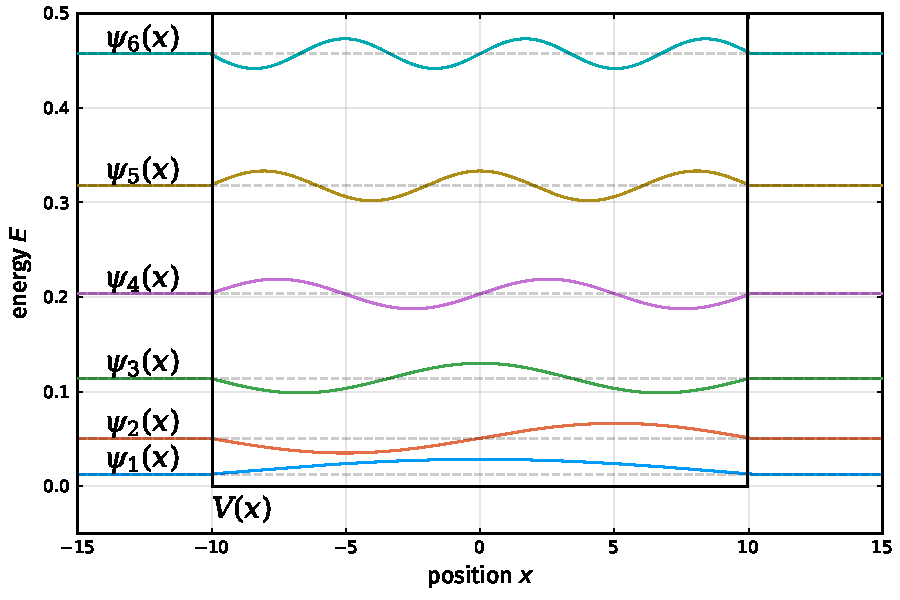
\includegraphics[width=0.8\textwidth]{figures/sec3_figures/infinite_well_eigenstates.pdf}
    \caption{无限深方势阱的能量本征态。}
\end{figure}

若已知系统零时刻处于几个能量本征态的叠加态,要求解系统波函数随时间的演化,将零时刻波函数投影至这些能量本征波函数之后,分别乘以相应的时间相位$\exp(-\ii E t/\hbar)$,重新相加即可。
一个运算技巧是先不要急于代入能量的表达式,而是先表为$E_n=n^2 E_1$,在化简完毕后再代入$E_1$的表达式。

若要求解系统的力学量平均值,直接使用相应算符在坐标表象下的表式求解即可,例如,坐标平均值
\begin{equation}
    \expval{x} = \mel{\psi}{x}{\psi} = \int_0^a \psi^*(x) \cdot x \psi(x) = \int_0^a x \abs{\psi(x)}^2;
\end{equation}
动量平均值
\begin{equation}
    \expval{p} = \mel{\psi}{p}{\psi} = \int_0^a \psi^*(x) \cdot -\ii\hbar\pd_x \psi(x);
\end{equation}
动量平方平均值
\begin{equation}
    \expval{p^2} = \mel{\psi}{p^2}{\psi} = \int_0^a \psi^*(x) \cdot -\hbar^2\pd_{xx}^2 \psi(x).
\end{equation}
注意,不少情况下,利用波函数的对称性及不同能级波函数的正交性可简化计算。

在计算的时候,也应熟记一些与三角函数有关的推论,例如二倍角与积化和差公式:
\begin{itemize}
    \item 二倍角公式
    \begin{equation}
    \begin{aligned}
        \sin 2\alpha &= 2\sin\alpha\cos\alpha, \\
        \cos 2\alpha &= \cos^2\alpha - \sin^2\alpha = 2\cos^2\alpha - 1 = 1 - 2\sin^2\alpha.
    \end{aligned}
    \end{equation}
    \item 积化和差公式
    \begin{equation}
    \begin{aligned}
        2\cos\alpha\cos\beta &= \cos(\alpha-\beta) + \cos(\alpha+\beta), \\
        2\sin\alpha\sin\beta &= \cos(\alpha-\beta) - \cos(\alpha+\beta), \\
        2\sin\alpha\cos\beta &= \sin(\alpha+\beta) + \sin(\alpha-\beta).
    \end{aligned}
    \end{equation}
\end{itemize}


% =================================================
\subsection{一维谐振子}
\label{subsec:onedim_osc}

我们设质量为$m$的物体受到$F=-kx$的弹性回复力,构成一维谐振子。

取平衡位置为原点,并利用圆频率$\omega\coloneq\sqrt{k/m}$,我们得到势能表式
\begin{equation}
    V(x) = \frac12 kx^2 = \frac12 m\omega^2 x^2,
\end{equation}
并进一步得到体系的Hamiltonian量
\begin{equation}
    \label{eq:onedim_osc_ham}
    H = \frac{p^2}{2m} + \frac12 m\omega^2 x^2.
\end{equation}

% ================================
\subsubsection{坐标表象}

在坐标表象下,可以写出一维谐振子的能量本征方程
\begin{equation}
    \left[ -\frac{\hbar^2}{2m}\pd_{xx}^2 + \frac12 m\omega^2 x^2 \right] \psi(x) = E\psi(x).
\end{equation}

作变量代换$\xi\coloneq \sqrt{m\omega/\hbar} x \coloneq \alpha x$,$\lambda = E/(\hbar\omega/2)$,
并作函数代换$\psi(\xi)=u(\xi)\ee^{-\xi^2/2}$,可得$u(\xi)$满足Hermite方程
\begin{equation}
    u''-2\xi u'+(\lambda-1)u = 0,
\end{equation}
可得满足波函数无穷远处渐近行为($\psi(x)\rightarrow 0$)的解为$u_n(\xi) = \rm{H}_n(\xi)$,
这里$\rm{H}_n(\xi)$是Hermite多项式,
对应的$\lambda=2n+1, n=0,1,2,\cdots$。

\begin{tcolorbox}
于是,就得到了一维谐振子体系的归一化能量本征函数及其对应的能量本征值:
\begin{equation}
    \label{eq:onedim_osc_coord_wfn}
    \psi_n(x) = \sqrt{\frac{\alpha}{2^n\cdot n! \sqrt{\pi}}} \rm{H}_n(\alpha x) \ee^{-\alpha^2 x^2/2}, \quad n=0,1,2,\cdots
\end{equation}
\begin{equation}
    E_n = \left(n+\frac12\right) \hbar\omega.
\end{equation}

特别地,对于基态,有
\begin{equation}
    \psi_0(x) = \sqrt{\frac{\alpha}{\sqrt{\pi}}} \ee^{-\alpha^2 x^2/2},
\end{equation}
\begin{equation}
    E_0 = \frac12 \hbar\omega.
\end{equation}
\end{tcolorbox}

\begin{figure}[ht]
    \centering
    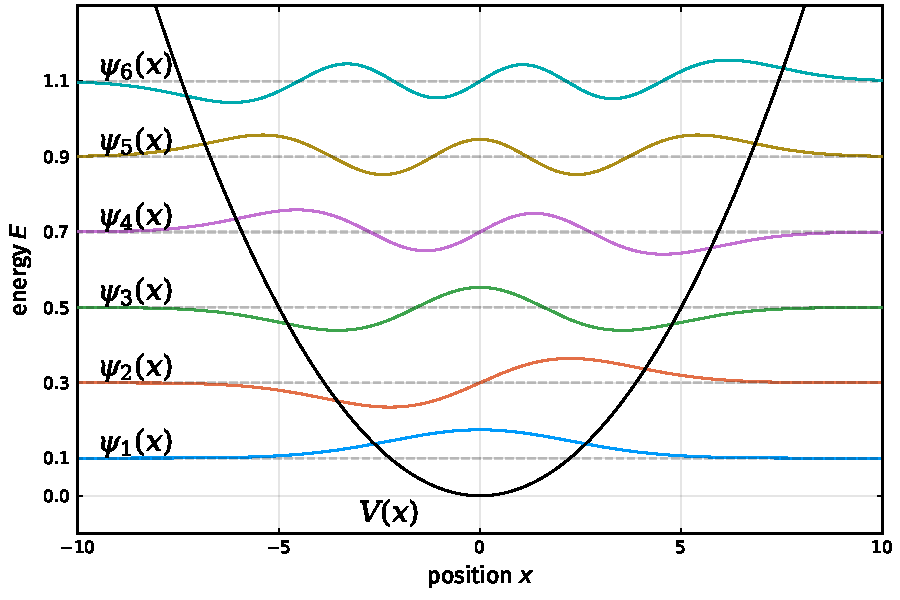
\includegraphics[width=0.8\textwidth]{figures/sec3_figures/harmonic_oscillator_eigenstates.pdf}
    \caption{一维谐振子的能量本征态。}
\end{figure}


% ================================
\subsubsection{粒子数表象}

我们注意到式\eqref{eq:onedim_osc_ham}中的坐标与动量算符的阶数均为二次,是对称的。
因此可以由此出发构建一组新的坐标,在新的表象下研究谐振子问题。

我们引入无量纲算符
\begin{equation}
    Q \coloneq \sqrt{\frac{m\omega}{\hbar}} x ,\quad P \coloneq \sqrt{\frac{1}{m\hbar\omega}} p,
\end{equation}
其对易子$[Q,P]=\ii$,
这样,Hamiltonian算符成为
\begin{equation}
    H = \frac12 \hbar\omega (Q^2+P^2).
\end{equation}

现我们定义算符
\begin{equation}
    a \coloneq \frac{1}{\sqrt{2}} (Q+\ii P) ,\quad a^\dag \coloneq \frac{1}{\sqrt{2}} (Q-\ii P),
\end{equation}
其对易子$[a,a^\dag]=1$。
我们发现
\begin{equation}
    a^\dag a = \frac12 (Q-\ii P)(Q+\ii P) = \frac{1}{\hbar\omega} H - \frac12,
\end{equation}
这就是说,
\begin{equation}
    H = (a^\dag a+\frac12)\hbar\omega.
\end{equation}
由$[a,a^\dag]=1$立刻得到
\begin{equation}
    H = (a a^\dag-\frac12)\hbar\omega
\end{equation}

我们假设谐振子按能量从低到高的第$n$($n=0,1,\cdots$)个能量为$E_n$的能量本征态为$\ket{n}$,然后考察$a,a^\dag$算符对能量本征态的影响。

我们研究$a\ket{n}$的能量本征值:
\begin{equation}
\begin{aligned}
    H a \ket{n}
    &= (a a^\dag - \frac12)\hbar\omega \cdot a \ket{n} \\
    &= (a a^\dag a - \frac12 a)\hbar\omega \ket{n} \\
    &= a (a^\dag a - \frac12)\hbar\omega \ket{n} \\
    &= a [(H-\hbar\omega) \ket{n}] \\
    &= (E_n-\hbar\omega) a \ket{n},
\end{aligned}
\end{equation}
可知$a\ket{n}$是$H$的另一个本征态,即能量本征值为$E_n-\hbar\omega$的能量本征态。
对能量本征态作用$a$一次,谐振子的能级下降$\hbar\omega$,因此$a$称为\emph{降算符}。
但能量不能无限下延,必须有基态能量$E_0$及对应本征态$\ket{0}$,使得$a\ket{0}$不再是本征态,为此我们可以置
\begin{equation}
    a \ket{0} = \bm{0}.
\end{equation}
借此,我们还可以求得基态能级:
\begin{equation}
    H\ket{0}
    = (a^\dag a+\frac12)\hbar\omega \ket{0}
    = \frac12\hbar\omega \ket{0}.
\end{equation}
这是说基态能级
\begin{equation}
    E_0 = \frac12 \hbar\omega.
\end{equation}

用类似的方法可以得到结论:$a^\dag\ket{n}$也是能量本征态,其能量本征值为$E_n+\hbar\omega$。
可见对能量本征态作用$a^\dag$将使得能级上升$\hbar\omega$,因此$a^\dag$称为\emph{升算符}。

在一些物理问题中,谐振子间传递的一份份能量可以看作一种称为声子的准粒子,能级的升降就对应着声子的创生和湮灭。
在量子光学中,电磁场量子化的结果是光子图像,光子的产生和湮灭也可以用升降算符表达。
因此,升/降算符又称\emph{产生(creation)/湮灭(annihilation)算符}。
另外,我们注意到$a^\dag a\ket{n}=\left(\frac{1}{\hbar\omega}H-\frac12\right)\ket{n}=n\ket{n}$,这就是说,算符
\begin{equation}
    N \coloneq a^\dag a
\end{equation}
对$\ket{n}$的本征值恰为量子数$n$,这一算符因此称为量子数/粒子数算符。
这也是这一表象名称(粒子数表象/Fock表象)的由来。

综上我们得到一维谐振子的全部能谱:
\begin{equation}
    E_n = \left(n+\frac12\right) \hbar\omega ,\quad n=0,1,2,\cdots.
\end{equation}

需要注意的是,$a$并非保留内积的幺正算符,因此$a\ket{n}\neq\ket{n-1}\ (n>0)$,而是$\lambda_n\ket{n-1}$。
通过归一条件$\braket{n}{n}=\braket{n-1}{n-1}=1$我们有
\begin{equation}
    \lambda_n^2 \braket{n-1}{n-1} = \mel{n}{a^\dag a}{n} = \mel{n}{\left(\frac{1}{\hbar\omega}H-\frac12\right)}{n} = n \braket{n}{n},
\end{equation}
于是我们得到$\lambda_n=\sqrt{n}$,进而
\begin{equation}
    a\ket{n} = \sqrt{n}\ket{n-1}.
\end{equation}
同理有
\begin{equation}
    a^\dag \ket{n} = \sqrt{n+1}\ket{n+1}.
\end{equation}
于是
\begin{equation}
\begin{aligned}
    \ket{1} &= a^\dag \ket{0}, \\
    \ket{2} &= \frac{1}{\sqrt{2}} (a^\dag)^2 \ket{0}, \\
    \ket{3} &= \frac{1}{\sqrt{3\cdot 2}} (a^\dag)^3 \ket{0}, \\
    \cdots \cdots \\
    \ket{n} &= \frac{1}{\sqrt{n!}} (a^\dag)^n \ket{0}.
\end{aligned}
\end{equation}

粒子数表象可以变换到坐标表象,从而求出谐振子的波函数。
写出升降算符在坐标表象中的表示
\begin{equation}
\begin{aligned}
    a       &= \frac{1}{\sqrt{2}}(Q+\ii P) = \frac{1}{\sqrt{2}}\left(\alpha x + \frac{1}{\alpha}\frac{\pd}{\pd x} \right), \\
    a^\dag  &= \frac{1}{\sqrt{2}}(Q-\ii P) = \frac{1}{\sqrt{2}}\left(\alpha x - \frac{1}{\alpha}\frac{\pd}{\pd x} \right).
\end{aligned}
\end{equation}
由$a\ket{0}=\bm{0}$在坐标表象下的表示
\begin{equation}
    a\ket{0} = \frac{1}{\sqrt{2}}\left(\alpha x + \frac{1}{\alpha}\frac{\pd}{\pd x} \right) \psi_0(x) = 0
\end{equation}
可以定出基态波函数,并利用归一化条件,可得
\begin{equation}
    \psi_0(x) = \sqrt{\frac{\alpha}{\sqrt{\pi}}} \ee^{-\alpha^2 x^2/2}.
\end{equation}
激发态波函数可以通过
\begin{equation}
    \ket{n} = \frac{1}{\sqrt{n!}} (a^\dag)^n \ket{0}
\end{equation}
定出,在坐标表象下,可得
\begin{equation}
    \psi_n(x) = \sqrt{\frac{\alpha}{2^n\cdot n! \sqrt{\pi}}} \left( \alpha x + \frac{1}{\alpha}\frac{\pd}{\pd x} \right)^n \ee^{-\alpha^2 x^2/2},
\end{equation}
如果我们引入$\xi=\alpha x$,并利用Hermite多项式满足的性质
\begin{equation}
    \rm{H}_n(\xi) = \ee^{\xi^2/2} \left( \xi + \frac{\pd}{\pd \xi} \right)^n \ee^{-\xi^2/2},
\end{equation}
我们就得到了坐标表象中的波函数(式\eqref{eq:onedim_osc_coord_wfn}),殊途同归。

\pagebreak
\section{时间演化}
\label{sec:time_evol}

在\ref{subsec:principles_time_evolution}节中,我们已经讨论了一个量子系统随时间演化的规律,
其中Schrödinger方程描述了量子态随时间的变化规律,而Heisenberg方程则描述了力学量(平均值)的演化规律。
事实上,量子态是无法直接观测的,我们所能直接观察的物理实在也仅仅是系统的可观测力学量。
从这个角度来说,Heisenberg方程显得更加自然并具有基础性。

% =================================================
\subsection{时间演化算符}

我们假定一个量子系统在零时刻与$t$时刻的量子态分别为$\ket{\psi(0)}$和$\ket{\psi(t)}$。
根据Schrödinger方程
\begin{equation}
    \ii\hbar\pd_t\ket{\psi} = H\ket{\psi},
\end{equation}
我们可以得到Schrödinger方程的一个形式解:
\begin{equation}
    \ket{\psi(t)} = \exp\left(-\ii \int_0^t H \dd\tau /\hbar\right)\ket{\psi(0)},
\end{equation}
若$H$不含时,则为
\begin{equation}
    \ket{\psi(t)} = \exp(-\ii H t/\hbar)\ket{\psi(0)}.
\end{equation}

我们看到,这个特殊的算符
\begin{equation}
    U(t,0) := \exp\left(-\ii \int_0^t H \dd\tau /\hbar\right)
\end{equation}
将两个时刻的量子态联系起来,称为\emph{时间演化算符(time-evolution operator)}
\footnote{倘若不同时刻的Hamiltonian不对易(即不总是满足$[H(t_1),H(t_2)]=0$),那么,时间演化算符的表式前要加上时间排序算符$𝒯$,其确保展开后的时间演化算符满足按时间顺序排列。}。
根据我们的物理直觉,这个算符显然具有\emph{幺正性(unitary)},即其是保留内积的变换,这是说
\begin{equation}
    \innerproduct{\psi(t)}{\psi(t)} = \mel{\psi(0)}{U^\dag U}{\psi(0)} = \mel{\psi(t)}{I}{\psi(0)} = \innerproduct{\psi(0)}{\psi(0)}.
\end{equation}
时间演化算符在形式上非常简单,然而在非对角的表象中,依然很难求出具体的形式。
\footnote{初学者可能对``算符的指数''存在误会。形式上,算符的指数可以直接按照指数函数的定义来理解,即$\exp A := \sum_{n=0}^\infty A^n/n!$。
    初学者可能认为``算符的指数的矩阵元''应该等于``原算符对应矩阵元的指数'',即$\{\exp A\}_{ij} = \exp(A_{ij})$,
    然而这是一种错误的观点(仅对``对角''算符成立),因为算符的指数是一个整体,它对整个算符进行指数运算,而不是对算符的每个元素分别进行指数运算。
}

在量子力学中,可观测力学量$F$的期望值是我们仅能直接观察的物理实在:
\begin{equation}
    \expval{F} = \mel{\psi(0)}{U^\dag F U}{\psi(0)},
\end{equation}
这个式子有两种不同的理解方式:
\begin{itemize}
    \item 第一种理解是认定力学量算符$F$保持不变,而量子态$\ket{\psi(t)}=U\ket{\psi(0)}$随时间演化,这就是说:
        \begin{equation}
            \expval{F} = \underbrace{\bra{\psi(0)}U^\dag}_{\bra{\psi(t)}} F \underbrace{U\ket{\psi(0)}}_{\ket{\psi(t)}},
        \end{equation}
        这种表述方式称为Schrödinger绘景(picture)。
    \item 第二种理解是认为力学量算符$F(t)=U^\dag F(0) U$随时间流易而演化,而量子态$\ket{\psi}$保持不变:
        \begin{equation}
            \expval{F} = \mel{\psi}{\underbrace{U^\dag F(0) U}_{F(t)}}{\psi}
        \end{equation}
        这种表述方式称为Heisenberg绘景。
\end{itemize}
两种绘景殊途同归,是完全等价的,在不同的问题中可以选择更适合的绘景进行分析。


% =================================================
\subsection{Virial定理}

我们研究一个位于势场$V(\rr)$中的粒子,其Hamiltonian:
\begin{equation}
    H = \frac{\pp^2}{2m} + V(\rr).
\end{equation}
对于定态,考察$\rr\cdot\pp$的期望值随时间的演化:
\begin{equation}
\begin{aligned}
    \frac{\dd}{\dd t}\expval{\rr\cdot\pp}
    &= \frac{1}{\ii\hbar} \expval{[\rr\cdot\pp, H]} \\
    &= \frac{1}{\ii\hbar} \expval{\rr\cdot[\pp,H] + [\rr,H]\cdot\pp}\\
    &= \frac{1}{\ii\hbar} \expval{-\ii\hbar\rr\cdot\nabla V(\rr) + \ii\hbar\pp^2/m} \\
    &= -\expval{\rr\cdot\nabla V(\rr)} + 2\expval{T},
\end{aligned}
\end{equation}
其中$T=\pp^2/2m$是动能。
对于定态,$\rr\cdot\pp$的期望值是一个常数,因此其时间导数为零,于是有
\begin{equation}
    2\expval{T} = \expval{\rr\cdot\nabla V(\rr)}.
\end{equation}
这就是\emph{Virial定理}。

这一定理对于特殊的势能函数具有特别的意义。
例如,对于$n$次齐次势能函数,有$\rr\cdot\nabla V(\rr) = nV(\rr)$,那么就有
\begin{equation}
    2\expval{T} = nV(\rr).
\end{equation}


% =================================================
\subsection{Ehrenfest定理}

对于一个量子波包,我们好奇的是,其坐标与动量随时间的变化率是否有与经典力学类似的形式?
我们设Hamiltonian为$H=\pp^2/2m + V(\rr)$,可以写出
\begin{equation}
\begin{aligned}
    \frac{\dd}{\dd t}\rr &= \frac{1}{\ii\hbar} \expval{[\rr, H]} = \frac{\expval{\pp}}{m}, \\
    \frac{\dd}{\dd t}\pp &= \frac{1}{\ii\hbar} \expval{[\pp, H]} = \expval{-\nabla V(\rr)} = \expval{\bm{F}(\rr)},
\end{aligned}
\end{equation}
可见这与经典力学Newton方程的形式非常相似,这就是\emph{Ehrenfest定理},其表明,量子波包的坐标与动量期望值的时间演化遵循类似经典力学的规律。


% =================================================
\subsection{Feynman-Hellmann定理}

Feynman-Hellmann定理指出,对于一个含参$\lambda$的Hamiltonian $H(\lambda)$,设$E_n$为其本征态$\ket{\psi_n}$的本征能量,则有
\begin{equation}
    \frac{\pd E_n}{\pd \lambda} = \mel{\psi_n}{\frac{\pd H}{\pd \lambda}}{\psi_n}.
\end{equation}

证明如下:
$E_n$为$H$的本征态$\ket{\psi_n}$的本征能量,因此有
\begin{equation}
    H\ket{\psi_n} = E_n \ket{\psi_n}.
\end{equation}
移项并对$\lambda$求导,得
\begin{equation}
    \left( \pd_\lambda H - \pd_\lambda E_n \right) \ket{\psi_n} + (H-E_n) \pd_\lambda \ket{\psi_n} = 0.
\end{equation}
左乘$\bra{\psi_n}$,并注意到$(H-E_n)\ket{\psi_n}=0$:
\begin{equation}
    \mel{\psi_n}{\pd_\lambda H - \pd_\lambda E_n}{\psi_n} + \underbrace{\bra{\psi_n} (H-E_n)}_{0} \pd_\lambda \ket{\psi_n} = 0.
\end{equation}
移项即得F-H定理,证毕。

\pagebreak

\section{全同粒子}
\label{sec:identical_particles}

全同粒子(identical particles)指不可区分的粒子,包含基本粒子(光子、电子、质子、中子)以及由基本粒子所组成的粒子,如原子核、原子、分子等。
本章我们将简单讨论全同粒子体系的量子态描述,以及全同粒子的交换对称性所带来的特殊情况。

% =================================================
\subsection{全同粒子量子态的描述}
\label{subsec:ip_state_desc}

我们考虑一由两个全同粒子组成的体系,在$q$表象下,体系的量子态$\ket{\Psi}$应同时由两个粒子各自的量子态$\ket{\psi}_1,\ket{\psi}_2$描述:
\begin{equation}
    \braket{\psi_{q_1},\psi_{q_2}}{\Psi} = \Psi_{q_1, q_2},
\end{equation}
这里的量子态$\ket{\psi_{q_1},\psi_{q_2}}=\ket{\psi_{q_1}}_1 \ket{\psi_{q_2}}_2$表示两个粒子中第一个处于$\ket{\psi_{q_1}}$,第二个处于$\ket{\psi_{q_2}}$的状态。
我们将看到,全同粒子体系的交换对称性将对体系的量子态提出一定要求,从而限制全同粒子体系实际波函数的形式。

% =================================================
\subsection{\texorpdfstring{交换对称性\quad Pauli不相容原理}{交换对称性  Pauli不相容原理}}
\label{subsec:ip_sym}

全同粒子体系的一大特点是\emph{“不可分辨”}。
这就是说,任何可观测量的测值概率分布在交换两个粒子时保持不变,称为\emph{“全同性原理”},是量子力学的基本公设之一。

我们考虑置换算符$P_{ij}$,其作用在于交换粒子$i,j$的全部坐标:
\begin{equation}
    P_{ij}\Psi(\cdots,q_i,\cdots,q_j,\cdots) = \Psi(\cdots,q_j,\cdots,q_i,\cdots),
\end{equation}
交换前后的量子态的力学量测值分布不应有变化,因此$\ket{\Psi}$与$P_{ij}\ket{\Psi}$最多只应当相差常数$C$。
我们设$P_{ij}\ket{\Psi}=C\ket{\Psi}$,并对$\ket{\Psi}$作用两次置换算符:
\begin{equation}
    P_{ij}^2\ket{\Psi} = C^2 \ket{\Psi},
\end{equation}
作用两次后,波函数应当复原,因此$C^2=1$,于是我们知道置换算符的本征态有两个,分别满足
\begin{equation}
\begin{aligned}
    P_{ij}\ket{\Psi}_{\rm{S}} &=  \ket{\Psi}_{\rm{S}}, \\
    P_{ij}\ket{\Psi}_{\rm{A}} &= -\ket{\Psi}_{\rm{A}}, \\
\end{aligned}
\end{equation}
前者的下标为Symmetric,称为\emph{对称量子态};
后者的下标为Anti-symmetric,称为\emph{反对称量子态}。

实验表明,全同粒子体系的量子态交换对称性与粒子自旋有着确定的联系。
凡自旋为整数倍$\hbar$的粒子,量子态是交换对称的,如$\pi$介子($s=0$)、$\alpha$粒子($s=0$)、光子($s=\hbar$),称为\emph{Bose子(Boson)};
凡自旋为半奇数倍$\hbar$的粒子,量子态是交换反对称的,如电子、质子和中子($s=\hbar/2$),称为\emph{Fermi子(Fermion)}。

满足交换对称/反对称原理的量子态如何构建?
我们考虑二粒子双本征态情形,设两个粒子能够分别处于单粒子态$\ket{\psi_{q_1}},\ket{\psi_{q_2}}$。

\paragraph{Bose子}
对于Bose子,量子态满足交换对称性,若$q_1\neq q_2$,我们可以将量子态写作归一化对称形式
\begin{equation}
    \ket{\psi_{q_1},\psi_{q_2}}_{\rm{S}}
    = \frac{1}{\sqrt{2}} (1+P_{12}) \left[\ket{\psi_{q_1}}_1 \ket{\psi_{q_2}}_2\right]
    = \frac{1}{\sqrt{2}} \left[\ket{\psi_{q_1}}_1 \ket{\psi_{q_2}}_2 + \ket{\psi_{q_2}}_1 \ket{\psi_{q_1}}_2\right],
\end{equation}
若$q_1=q_2=q$,则
\begin{equation}
    \ket{\psi_{q},\psi_{q}}_\rm{S} = \ket{\psi_q}_1 \ket{\psi_q}_2.
\end{equation}

\paragraph{Fermi子}
对于Fermi子,量子态满足交换反对称性,若$q_1\neq q_2$,有
\begin{equation}
    \ket{\psi_{q_1},\psi_{q_2}}_{\rm{A}}
    = \frac{1}{\sqrt{2}} (1-P_{12}) \left[\ket{\psi_{q_1}}_1 \ket{\psi_{q_2}}_2\right]
    = \frac{1}{\sqrt{2}}
    \begin{vmatrix}
        \ket{\psi_{q_1}}_1 & \ket{\psi_{q_1}}_2 \\
        \ket{\psi_{q_2}}_1 & \ket{\psi_{q_2}}_2
    \end{vmatrix},
\end{equation}
这种形式称为\emph{Slater行列式};
若$q=q_1=q_2$,则
\begin{equation}
    \ket{\psi_q,\psi_q}_{\rm{A}} = 0.
\end{equation}
这说明\emph{两个全同Fermi子不能同时处于同一个单粒子态,称为Pauli不相容原理。}

\begin{tcolorbox}[breakable, colframe=purple, colback=red!10, title={\textbf{Bose, Fermi与经典体系粒子的组合数计算}}]
    \it\small
    一个常见的问题是计算Bose, Fermi与经典体系粒子的组合数:
    $n$个全同粒子处于$m$个可能的单粒子态,对于Bose子, Fermi子与经典粒子,可能有几种组合方式?

    对于经典粒子,粒子是完全可分辨的,因此粒子间互不相关,可能的组合数有
    \begin{equation}
        N_{\rm{classical}} = m^n.
    \end{equation}

    对于Bose子,粒子不可分辨,可以用隔板法求取可能的组合数:
    设置$m-1$个隔板,与$n$个粒子混合排列,这样$n$个粒子就被隔板分至$m$个态上,有$(n+m-1)!$种方式。
    隔板与粒子分别不可分辨,因此除以各自排列数$(m-1)!$与$n!$
    \begin{equation}
        N_{\rm{Bose}} = \frac{(n+m-1)!}{(m-1)! n!}.
    \end{equation}

    对于Fermi子,粒子不可分辨,且是互斥的,于是从$m\ (m>n)$个态中选取$n$个分别放入一个粒子即可,可能的组合数:
    \begin{equation}
        N_{\rm{Fermi}} = P_m^n = \frac{m!}{n!(m-n)!}.
    \end{equation}

\end{tcolorbox}

\pagebreak

\section{中心力场}
\label{sec:central_field}

中心力场是一种势能仅与$r$有关的力场,势能可以写作$V(r)$。
写出在中心势$V(r)$中质量为$m$的粒子的Hamiltonian算符
\begin{equation}
    H = \frac{p^2}{2m} + V(r).
\end{equation}
可以证明角动量是守恒量:$[\bm{l},H]=\bm{0}$,这与经典力学的结论是一致的。

在坐标表象、球坐标下求解中心力场问题一般较为方便。
写出Hamiltonian算符在坐标表象、球坐标中的形式,定态\schrodinger 方程可以分离出径向和角向部分,定态波函数解也可以被表为径向和角向分离变量的形式:
\begin{equation}
    \psi(r,\theta,\phi) = R(r) \rm{Y}_{lm}(\theta,\phi),\quad l=0,1,2,\cdots,\ m=-l,-l+1,\cdots,l,
\end{equation}
其中$Y_{lm}$是球谐函数,是$l^2$与$l_z$的共同本征函数;
径向函数$R(r)$满足方程
\begin{equation}
    R_l'' + \frac{2}{r} R_l' + \left[\frac{2m}{\hbar^2}(E-V(r))-\frac{l(l+1)}{r^2}\right] R_l = 0,
\end{equation}
可见在中心力场中,粒子波函数的差别仅在于径向部分。
选取一定的边界条件求解径向方程,对于束缚态($E<\lim_{r\rightarrow\infty} V(r)$),可得到径向量子数$n_r$及其对应的能量本征值$E_{n_r l}$。
径向方程中不出现$m$,说明$E$与$m$无关,即中心力场中每个能级都至少有$m$个\emph{简并(degenerate)}的量子态。

如此,我们选用了$\{H, l^2, l_z\}$作为描述中心力场量子态的力学量集,并用$n_r, l, m$(径向量子数、角量子数\footnote{$l=0,1,2,3$分别对应字母s,p,d,f,而之后沿字母表顺延。}与磁量子数)三个量子数区分这些量子态。
这一力学量集足以区分各个简并的量子态,而且是“适定”的,因此称为\emph{力学量完全集}。

% =================================================
\subsection{三维各向同性球谐振子}
\label{subsec:cf_osc}

我们考虑一个质量为$m$、位于三维各向同性谐振子势
\begin{equation}
    V(r) = \frac12 m\omega^2 r^2
\end{equation}
中的粒子。

求解径向方程,利用无穷远处$R(r)\rightarrow 0$的边界条件,我们得到了能量本征值
\begin{equation}
    E = \left( 2n_r+l+\frac32 \right)\hbar\omega,\quad n_r,l=0,1,2,\cdots
\end{equation}
取$N=2n_r+l$,能量本征值写为
\begin{equation}
    E_N = (N+\frac32) \hbar\omega,\quad N=0,1,2,\cdots.
\end{equation}
可以发现,与一维谐振子相同,三维各向同性球谐振子的能级是均匀分布的,间距为$\hbar\omega$,不过零点能为$\frac32\hbar\omega$。

可以求解出对于给定的能级$E_N$,有多少可能的量子态(用$n_r,l,m$区分)共享同一个能级,即简并度是多少。
我们知道,对于给定的$N$,可能的$(n_r,l)$组合有
\begin{equation}
    (0,N),\ (1,N-2),\ (2,N-4)\cdots\cdots
    \begin{cases}
        ((N-1)/2, 1),   & \rm{for\ odd\ }N, \\
        (N/2, 0)        & \rm{for\ even\ }N, \\
    \end{cases}
\end{equation}
对于每一组$(n_r,l)$,都有$2l+1$个不同的$m$的量子态,因此简并度
\begin{equation}
    d_N =
    \begin{cases}
        \sum_{l=1,3,\cdots,N} = \frac12 (N+1)(N+2), & \rm{for\ odd\ }N, \\
        \sum_{l=0,2,\cdots,N} = \frac12 (N+1)(N+2), & \rm{for\ even\ }N. \\
    \end{cases}
\end{equation}
可见,对于奇数或者偶数的$N$,简并度均为
\begin{equation}
    d_N = \frac12 (N+1)(N+2).
\end{equation}

我们看到,三维各向同性球谐振子场具有比一般中心力场更高的简并度,这与其径向势场有关,更高的“对称性”导致了更多的简并态。

% =================================================
\subsection{氢原子}
\label{subsec:cf_hydrogen}

氢原子中有一个质子和电子,故其实际上是一个两体问题。
可以通过引入质心坐标和相对坐标的方法,将两体问题化为单体问题。
这样,仍然可以沿用之前的中心力场的处理方法,但质量需理解为约化质量,能量理解为相对运动能量。

在自然单位制$\hbar=m_e=\abs{e}=1$下,Coulomb势场的能量为
\begin{equation}
    V(r) = -\frac{1}{r}.
\end{equation}

由径向方程的边界条件,给出径向量子数$n_r=0,1,2,\cdots$,本征能量为
\begin{equation}
    E_n = -\frac{1}{2(n_r+l_1)^2},
\end{equation}
取主量子数$n:=n_r+l_1+1,\ n=1,2,\cdots$,可得
\begin{equation}
    E_n = -\frac{1}{2n^2}.
\end{equation}

能量的自然单位为$me^4/\hbar^2 = 1\ \rm{Hartree} \approx 27.211\ \rm{eV}$,
长度的自然单位是$a_0 = \hbar^2/me^2 \approx 0.529\ \rm{Å}$,为一个Bohr半径。
如此,本征能量表为
\begin{equation}
    E_n = -\frac{e^2}{a_0}\frac{1}{2n^2},
\end{equation}
其中基态的能量为$E_1 = -\frac{e^2}{a_0} \approx -13.6\ \rm{eV}$。

我们用$(n,l,m)$来区分氢原子的各个量子态。
\begin{itemize}
    \item 角动量平方的期望值$\expval{\LL^2}=l(l+1)\hbar^2$;
    \item 角动量$z$分量的期望值$\expval{L_z}=m\hbar$。
\end{itemize}

特别地,我们写出基态的波函数:
\begin{equation}
    \psi_{100}(r) = \frac{1}{\sqrt{\pi a_0^3}}\ee^{-r/a_0}.
\end{equation}
读者应牢记。

最后还有一个计算技巧。
在计算$r^n$的期望值时,可以采用如下的策略:
\begin{equation}
\begin{aligned}
    \expval{r^n}
    &= \frac{\int r^2 \dd r \dd\Omega \ Y_{lm}^*(\theta,\phi) r^n Y_{lm}(\theta,\phi) R_{nl}^2(r)}{\int r^2 \dd r \dd\Omega \ Y_{lm}^*(\theta,\phi) Y_{lm}(\theta,\phi) R_{nl}^2(r)} \\
    &= \frac{\int\dd r \ r^{n+2} R_{nl}^2(r)}{\int\dd r \ r^2 R_{nl}^2(r)},
\end{aligned}
\end{equation}
其中$R_{nl}(r)$是多项式$P(r)$与$\ee^{-r/na_0}$的乘积,因此问题最后可以归结为求解一个重要积分:
\begin{equation}
    \int_0^\infty \dd t \ t^{N} \ee^{-t} = \Gamma(N+1) = N!,
\end{equation}
这一公式需牢记。

\pagebreak
\section{自旋}
\label{sec:spin}

% % =================================================
% \subsection{自旋-1/2体系的Pauli表象}
% \label{subsec:spin_single_particle}

电子除了空间上的三个自由度,还有一个内禀(intrinsic)属性——\emph{自旋(spin)},用$\bm{s}$表示。
根据Stern-Gerlach实验,电子的自旋投影具有二值性,即只能取$s_z=+\hbar/2$或$s_z=-\hbar/2$。

自旋具有角动量的特征,因此我们假定其具备与角动量类似的量子性质,其对易关系满足:
\begin{equation}
    [s_i,s_j]=\ii\hbar\epsilon_{ijk}s_k.
\end{equation}
再引入无量纲自旋Pauli算符
\begin{equation}
    \bm{\sigma}=\bm{s}/\frac{\hbar}{2},
\end{equation}
对易关系成为:
\begin{equation}
    [\sigma_i,\sigma_j]=2\ii\epsilon_{ijk}\sigma_k.
\end{equation}
其还满足
\begin{equation}
    \sigma_i^2 = 1, \quad
    \sigma_i\sigma_j = \ii \epsilon_{ijk}\sigma_k \quad (i\ne j).
\end{equation}

Pauli表象选取$s_z=\pm\hbar/2$(即$\ket{\up},\ket{\down}$)的本征态作为描述系统状态的基矢。
在这一表象下,Pauli算符的各个分量为:
\begin{equation}
    \sigma_z = \begin{pmatrix}1& 0\\0&-1\end{pmatrix}, \quad
    \sigma_x = \begin{pmatrix}0& 1\\1& 0\end{pmatrix}, \quad
    \sigma_y = \begin{pmatrix}0&-\ii\\ \ii& 0\end{pmatrix}.
\end{equation}

\begin{tcolorbox}[breakable, title={\textbf{例题}}]
    \paragraph{题目} \textit{(2019年考研·六)}
    电子处于沿$z$轴方向,磁感应强度为$B_0 \cos\omega t$的时变磁场中。零时刻测得其自旋$x$分量为$+\hbar/2$。
    求$t$时刻的量子态。

    \paragraph{解答}
    我们在Pauli表象下研究这个问题。

    首先求出零时刻量子态在Pauli表象下的表示$\chi_0^{(s_z)}$,其为$\sigma_x$的本征值为$+1$的本征态。
    $\sigma_x$的矩阵形式为
    \begin{equation}
        \sigma_x^{(s_z)} = \begin{pmatrix} & 1 \\ 1 & \end{pmatrix},
    \end{equation}
    于是得到零时刻量子态
    \begin{equation}
        \chi_0^{(s_z)} = \frac{1}{\sqrt{2}} \begin{pmatrix} 1 \\ 1 \end{pmatrix}.
    \end{equation}

    接下来,我们写出Hamiltonian:
    \begin{equation}
        H = -\mu_{\rm{B}} B(t) \sigma_z = - \underbrace{\frac{e\hbar}{2m_e} B_0}_{E_0} \cos\omega t \sigma_z,
    \end{equation}
    其中$\mu_{\rm{B}}$是Bohr磁子。

    量子态的演化满足Schrödinger方程,我们设$\chi^{(s_z)}(t)=[\chi_a(t), \chi_b(t)]^T$,那么有
    \begin{equation}
        \ii\hbar\pd_t \begin{pmatrix}\chi_a \\ \chi_b \end{pmatrix}
        = H \begin{pmatrix} \chi_a \\ \chi_b \end{pmatrix}
        = \begin{pmatrix} -E_0 \cos\omega t \chi_a \\ E_0 \cos\omega t \chi_b \end{pmatrix},
    \end{equation}
    于是得到两个分离的常微分方程
    \begin{equation}
        \ii\hbar\pd_t \chi_a = -E_0 \cos\omega t \chi_a,\quad
        \ii\hbar\pd_t \chi_b =  E_0 \cos\omega t \chi_b,
    \end{equation}
    解之,并用初条件$\chi_a(0)=1/\sqrt2,\ \chi_b(0)=1/\sqrt2$定解,就得到$t$时刻的量子态
    \begin{equation}
        \chi_a(t) = \frac{1}{\sqrt{2}} \ee^{\ii\frac{E_0}{\hbar\omega}\sin\omega t},\quad
        \chi_b(t) = \frac{1}{\sqrt{2}} \ee^{-\ii\frac{E_0}{\hbar\omega}\sin\omega t}.
    \end{equation}
    \hfill$\square$
\end{tcolorbox}

在Hamiltonian不含时的情形中,若Hamiltonian能表为$\bm{\sigma}$的分量的线性组合(例如:$H=E_0\sigma_i$),可利用结论
\begin{equation}
    \label{eq:spin_exp_pauli}
    \ee^{\ii \bm{\alpha}\cdot\bm{\sigma}} = \cos\alpha + \ii \sin\alpha (\hat{\bm{\alpha}}\cdot\bm{\sigma}),
\end{equation}
而无需变换至$\sigma_i$表象。
该结论可利用$\ee^{\ii \bm{\alpha}\cdot\bm{\sigma}}$的Taylor展开式证明:
\begin{equation}
\begin{aligned}
    \ee^{\ii \bm{\alpha}\cdot\bm{\sigma}}
    &= \sum_{n=0}^\infty \frac{(\ii \bm{\alpha}\cdot\bm{\sigma})^n}{n!}\\
    &= \sum_{n=0}^\infty \frac{(-1)^n (\bm{\alpha}\cdot\bm{\sigma})^{2n}}{(2n)!} + \ii \sum_{n=0}^\infty \frac{(-1)^n (\bm{\alpha}\cdot\bm{\sigma})^{2n+1}}{(2n+1)!}\\
    &= \sum_{n=0}^\infty \frac{(-1)^n \alpha^{2n}}{(2n)!} + \ii (\hat{\alpha}\cdot\sigma) \sum_{n=0}^\infty \frac{(-1)^n \alpha^{2n+1}}{(2n+1)!}\\
    &= \cos\alpha + \ii \sin\alpha (\hat{\alpha}\cdot\bm{\sigma}).
\end{aligned}
\end{equation}

\begin{tcolorbox}[breakable, title={\textbf{例题}}]
    \paragraph{题目} \textit{(2023年考研·五)}
    电子处于沿$x$轴方向,磁感应强度为$B_0$的静磁场中。零时刻测得其自旋$z$分量为$+\hbar/2$。
    求:\\
    (1) $t$时刻的量子态;\\
    (2) $t$时刻电子自旋各个分量的期望值。

    \paragraph{解答}
    Hamiltonian为
    \begin{equation}
        H = -\mu_{\rm{B}} B_0 \sigma_x = - \underbrace{\frac{e\hbar}{2m_e} B_0}_{E_0} \sigma_x,
    \end{equation}
    则$0\rightarrow t$的时间演化算符为
    \begin{equation}
        U(t,0) = \ee^{-\ii H t/\hbar} = \ee^{\ii E_0 \sigma_x t/\hbar},
    \end{equation}
    $t$时刻与零时刻的量子态通过时间演化算符相联系:
    \begin{equation}
        \ket{\psi(t)} = U(t,0) \ket{\psi(0)} = \ee^{\ii E_0 \sigma_x t/\hbar} \ket{\psi_0}
        = \cos(E_0 t/\hbar)\ket{\psi_0} + \sin(E_0 t/\hbar) \sigma_x \ket{\psi_0}.
    \end{equation}

    现在,我们在Pauli表象下写出$\ket{\psi(0)}$和$\ket{\psi(t)}$的具体表式。
    零时刻态为$s_z=\hbar/2$的本征态:
    \begin{equation}
        \psi^{(s_z)}(0) = \begin{pmatrix} 1 \\ 0 \end{pmatrix},
    \end{equation}
    代入上式,我们得到$t$时刻态的表示为
    \begin{equation}
        \psi^{(s_z)}(t) = \cos(E_0 t/\hbar)\begin{pmatrix} 1 \\ 0 \end{pmatrix} + \sin(E_0 t/\hbar) \underbrace{\begin{pmatrix} 0 & 1 \\ 1 & 0 \end{pmatrix}}_{\sigma_x} \begin{pmatrix} 1 \\ 0 \end{pmatrix}
        = \begin{pmatrix} \cos(E_0 t/\hbar) \\ \sin(E_0 t/\hbar) \end{pmatrix}.
    \end{equation}

    自旋各分量的期望值为:
    \begin{equation}
    \begin{aligned}
        \expval{s_z}(t) &= \mel{\psi(t)}{s_z}{\psi(t)} \\
        &= \frac{\hbar}{2} \begin{pmatrix} \cos(E_0 t/\hbar) & \sin(E_0 t/\hbar) \end{pmatrix} \begin{pmatrix} 1 & \\ & -1 \end{pmatrix} \begin{pmatrix} \cos(E_0 t/\hbar) \\ \sin(E_0 t/\hbar) \end{pmatrix} \\
        &= \frac{\hbar}{2} \left(\cos^2(E_0 t/\hbar) - \sin^2(E_0 t/\hbar)\right)
        = \frac{\hbar}{2} \cos(2E_0 t/\hbar); \\
        \expval{s_x}(t) &= \mel{\psi(t)}{s_x}{\psi(t)} = \frac{\hbar}{2} \sin(2E_0 t/\hbar); \\
        \expval{s_y}(t) &= \mel{\psi(t)}{s_y}{\psi(t)} = 0.
    \end{aligned}
    \end{equation}
    \hfill $\square$
\end{tcolorbox}

\pagebreak
\section{角动量}
\label{sec:angular_momentum}

% % =================================================
% \subsection{角动量算符}
% \label{subsec:angular_momentum_ops}

在这一节中,我们将讨论量子力学中的角动量算符以及描述角动量表象的代数方法。

我们从最基本的角动量算符对易关系开始:
\begin{equation}
    [L_i, L_j] = \ii\hbar\epsilon_{ijk}L_k.
\end{equation}
从这个对易关系,我们发现
\begin{equation}
    [L^2, L_i] = 0,
\end{equation}
这表明$L^2$与$L_i$拥有共同本征态,因此可以作为一组角动量表象下描述量子态的对易力学量集合,这里我们选取$i=z$。

我们设想用$l,m$作为描述$L^2,L_z$的本征态的量子数,用$\ket{lm}$表示。
假定$L^2,L_z$的量子数为$l,m$的本征态对应的本征值分别为$\lambda\hbar^2$和$m\hbar$,即:
\begin{equation}
\begin{aligned}
    L^2\ket{lm} &= \lambda\hbar^2\ket{lm} \\
    L_z\ket{lm} &= m\hbar\ket{lm}, \quad m=\cdots -1, 0, 1, \cdots.
\end{aligned}
\end{equation}
这里$m$的取值我们暂时仅仅限定为整数,这一结论可以由$L_z$在球坐标系中的本征态需要满足周期性边界条件确定,而进一步限定$m$的取值范围则需后续讨论。

我们发现,一维谐振子的升降算符法同样可以应用于角动量问题。
角动量表象下的\emph{升降算符}定义为:
\begin{equation}
    L_\pm := L_x \pm \ii L_y.
\end{equation}

首先来研究一下升降算符的性质:
\begin{equation}
    [L_z, L_\pm] = [L_z, L_x \pm \ii L_y] = \pm\hbar L_\pm ,\quad
    [L^2, L_\pm] = 0, \quad
    [L_+, L_-] = 2\hbar L_z;
\end{equation}
\begin{equation}
    L_\pm L_\mp = L_x^2 + L_y^2 \pm \ii[L_y, L_x] = L_x^2 + L_y^2 \pm \hbar L_z = L^2 - L_z^2 \pm \hbar L_z.
\end{equation}

现在,我们来考察升降算符作用在量子态上的情况,我们发现:
\begin{equation}
    L_z L_\pm \ket{lm}
    = (\red{L_\pm L_z} + \blue{[L_z, L_\pm]}) \ket{lm}
    = (\red{(L_\pm m\hbar)} \blue{\pm (\hbar L_\pm)}) \ket{lm}
    = (\red{m}\blue{\pm 1})\hbar L_\pm \ket{lm},
\end{equation}
这意味着$L_\pm\ket{lm}$也是$L_z$的本征态,且对应的本征值为$(m\pm 1)\hbar$。
此外,由于$[L^2, L_\pm] = 0$,可以得知$L_\pm\ket{lm}$对应的$L^2$本征值与$\ket{lm}$的相同。
这就是说
\begin{equation}
    L_\pm \ket{lm} = c_{lm}^{(\pm)} \ket{l,m\pm 1},
\end{equation}
即升降算符将使得角动量分量$L_z$增加或减少$\hbar$,而不会改变角动量平方值$L^2$。

直到目前,我们尚未明确$\lambda$与$l$的关系。
这一关系可以借助角动量作为一个矢量所满足的限制条件来确定:
\begin{equation}
    L_z^2 \leq L^2, \ \text{i.e.,}\ m^2 \leq \lambda.
\end{equation}
这就是说,对于给定的$l$(对应一个确定的$\lambda$),$m$的取值有确定的上下限$\pm m_{\text{max}}$。
我们不妨置$l=m_{\text{max}}$,那么,对于$m=l$的量子态$\ket{ll}$,升算符作用后的状态应不存在,这就是说
\begin{equation}
    L_+ \ket{ll} = 0.
\end{equation}
左乘以$L_-$,我们发现
\begin{equation}
    L_- L_+ \ket{ll} = (L^2 - L_z^2 - \hbar L_z) \ket{ll} = [\lambda - l(l+1)]\hbar^2 \ket{ll} = 0,
\end{equation}
这意味着
\begin{equation}
    \lambda = l(l+1),
\end{equation}
即$\ket{lm}$态的$L^2$的本征值是$l(l+1)\hbar^2$。

现在,我们成功地用代数方法获得了角动量表象的态空间以及对应的力学量本征值:
\begin{equation}
    L^2 \ket{lm} = l(l+1)\hbar^2 \ket{lm},\quad l=0,1,\ldots,
    L_z \ket{lm} = m\hbar \ket{lm},\quad m=-l,-l+1,\ldots,l.
\end{equation}

最后,我们再来推导升降算符的矩阵元。
注意到$L_+ L_-$作用于$\ket{lm}$时,得到的应当是$\ket{lm}$的相应倍数:
\begin{equation}
    L_+ L_- \ket{lm} = c_{l,m-1}^{(+)} c_{lm}^{(-)} \ket{lm},
\end{equation}
又注意到$L_+^\dag=L_-$,因此
\begin{equation}
    c_{lm}^{(-)} = \mel{l,m-1}{L_-}{lm} = \mel{l,m}{L_+}{lm} = c_{l,m+1}^{(+)},
\end{equation}
所以我们得到$L_+ L_-$的矩阵元为
\begin{equation}
    \mel{lm}{L_+ L_-}{lm} = c_{lm}^{(-)2} = c_{l,m-1}^{(+)2}.
\end{equation}
我们再利用$L_+ L_- = L^2 - L_z^2 + \hbar L_z$,有
\begin{equation}
    \mel{lm}{L_+ L_-}{lm} = [l(l+1) - m(m-1)] \hbar^2.
\end{equation}
对比以上两式,我们就得到升降算符的矩阵元
\begin{equation}
\begin{aligned}
    c_{lm}^{(-)} &= \mel{l,m-1}{L_-}{lm} = \sqrt{l(l+1) - m(m-1)} \hbar = \sqrt{(l+m)(l-m+1)} \hbar,\\
    c_{lm}^{(+)} &= \mel{l,m+1}{L_+}{lm} = \sqrt{l(l+1) - m(m+1)} \hbar = \sqrt{(l-m)(l+m+1)} \hbar,
\end{aligned}
\end{equation}
这里矩阵元的正负号可利用$L_+\ket{ll}=0$与$L_-\ket{l-l}=0$助记。

至于$L_x, L_y$的矩阵元,可利用
\begin{equation}
    L_x = \frac12 (L_+ + L_-), \quad L_y = \frac{1}{2\ii} (L_+ - L_-)
\end{equation}
求解:
\begin{equation}
\begin{aligned}
    \mel{l,m+1}{L_x}{lm} &= \frac12 c_{lm}^{(+)},\\
    \mel{l,m-1}{L_x}{lm} &= \frac12 c_{lm}^{(-)},\\
    \mel{l,m+1}{L_y}{lm} &= \frac{1}{2\ii} c_{lm}^{(+)},\\
    \mel{l,m-1}{L_y}{lm} &= -\frac{1}{2\ii} c_{lm}^{(-)}.
\end{aligned}
\end{equation}

\begin{tcolorbox}[breakable, title={\textbf{例题}}]
    \paragraph{题目} \textit{(2019年考研·四)}
    对于$\ket{lm}$态,求:\\
    (1) $\expval{L_x}, \expval{L_y}$;\\
    (2) $\expval{\Delta L_x^2}, \expval{\Delta L_y^2}$。

    \paragraph{解答}
    (1) 我们知道
    \begin{equation}
        \mel{lm}{L_+}{lm} = c_{lm}^{(+)} \braket{lm}{l,m+1} = 0, \quad
        \mel{lm}{L_-}{lm} = c_{lm}^{(-)} \braket{lm}{l,m-1} = 0,
    \end{equation}
    而$L_x, L_y$为$L_+, L_-$的线性组合,因此其对角矩阵元均为零:
    \begin{equation}
        \expval{L_x} = \mel{lm}{L_x}{lm} = 0, \quad
        \expval{L_y} = \mel{lm}{L_y}{lm} = 0.
    \end{equation}
    (2) 以$\Delta L_x^2$为例。
    由于$\expval{\Delta L_x^2}=\expval{L_x^2}-\expval{L_x}^2=\expval{L_x^2}$,仅需计算$L_x^2$的对角矩阵元。
    我们写出$L_x^2$关于升降算符的表达式:
    \begin{equation}
        L_x^2 = \frac14 (L_+ + L_-)^2 = \frac14 (L_+^2 + L_-^2 + L_+ L_- + L_- L_+).
    \end{equation}
    显然,仅有$L_+ L_- + L_- L_+$项的对角矩阵元非零:
    \begin{equation}
    \begin{aligned}
        \mel{lm}{L_+ L_-}{lm} &= c_{lm}^{(-)2} = \sqrt{l(l+1)-m(m-1)}\hbar^2, \\
        \mel{lm}{L_- L_+}{lm} &= c_{lm}^{(+)2} = \sqrt{l(l+1)-m(m+1)}\hbar^2.
    \end{aligned}
    \end{equation}
    因此
    \begin{equation}
        \expval{\Delta L_x^2} = \frac14 (c_{lm}^{(-)2} + c_{lm}^{(+)2}) = \frac12 [l(l+1)-m^2]\hbar^2.
    \end{equation}
    同理可得
    \begin{equation}
        \expval{\Delta L_y^2} = \expval{\Delta L_x^2} = \frac12 [l(l+1)-m^2]\hbar^2.
    \end{equation}
    \hfill $\square$
\end{tcolorbox}

\pagebreak

\end{document}
